%%
%% This is file `sample-authordraft.tex',
%% generated with the docstrip utility.
%%
%% The original source files were:
%%
%% samples.dtx  (with options: `authordraft')
%% 
%% IMPORTANT NOTICE:
%% 
%% For the copyright see the source file.
%% 
%% Any modified versions of this file must be renamed
%% with new filenames distinct from sample-authordraft.tex.
%% 
%% For distribution of the original source see the terms
%% for copying and modification in the file samples.dtx.
%% 
%% This generated file may be distributed as long as the
%% original source files, as listed above, are part of the
%% same distribution. (The sources need not necessarily be
%% in the same archive or directory.)
%%
%% Commands for TeXCount
%TC:macro \cite [option:text,text]
%TC:macro \citep [option:text,text]
%TC:macro \citet [option:text,text]
%TC:envir table 0 1
%TC:envir table* 0 1
%TC:envir tabular [ignore] word
%TC:envir displaymath 0 word
%TC:envir math 0 word
%TC:envir comment 0 0
%%
%%
%% The first command in your LaTeX source must be the \documentclass command.
% \documentclass[sigconf,review,anonymous]{acmart}
% \documentclass[sigconf,review, anonymous]{acmart}
\documentclass[sigconf]{acmart}
%% NOTE that a single column version may required for 
%% submission and peer review. This can be done by changing
%% the \doucmentclass[...]{acmart} in this template to 
%% \documentclass[manuscript,screen]{acmart}
%% 
%% To ensure 100% compatibility, please check the white list of
%% approved LaTeX packages to be used with the Master Article Template at
%% https://www.acm.org/publications/taps/whitelist-of-latex-packages 
%% before creating your document. The white list page provides 
%% information on how to submit additional LaTeX packages for 
%% review and adoption.
%% Fonts used in the template cannot be substituted; margin 
%% adjustments are not allowed.

%%
%% \BibTeX command to typeset BibTeX logo in the docs
\AtBeginDocument{%
  \providecommand\BibTeX{{%
    \normalfont B\kern-0.5em{\scshape i\kern-0.25em b}\kern-0.8em\TeX}}}


%% use packages:
\usepackage{enumitem}
\usepackage{multirow}
\usepackage{subfig}
\usepackage{soul}
\usepackage{balance}

\newenvironment{packed_lefty_item}{
\begin{itemize}[leftmargin=*]
\vspace{-2pt}
  \setlength{\itemsep}{0pt}
  \setlength{\parskip}{0pt}
  \setlength{\parsep}{0pt}
  \setlength{\topsep}{-10pt}
  \setlength{\partopsep}{0pt}
}{\end{itemize}\vspace{-2pt}}

%% Rights management information.  This information is sent to you
%% when you complete the rights form.  These commands have SAMPLE
%% values in them; it is your responsibility as an author to replace
%% the commands and values with those provided to you when you
%% complete the rights form.

\copyrightyear{2024}
\acmYear{2024}
\setcopyright{acmlicensed}
\acmConference[MM '24] {Proceedings of the 32nd ACM International Conference on Multimedia}{October 28--November 1, 2024}{Melbourne, VIC, Australia.}
\acmBooktitle{Proceedings of the 32nd ACM International Conference on Multimedia (MM '24), October 28--November 1, 2024, Melbourne, VIC, Australia}
\acmISBN{979-8-4007-0686-8/24/10}
\acmDOI{10.1145/XXXXXX.XXXXXX}

\settopmatter{printacmref=true}  
% \settopmatter{printacmref=false} % Removes citation information below abstract
% \renewcommand\footnotetextcopyrightpermission[1]{} % removes footnote with conference information in first column
% \pagestyle{plain} % removes running headers 
% \setcopyright{none}

% remove footnote
% \renewcommand\footnotetextcopyrightpermission[1]{}

%% These commands are for a PROCEEDINGS abstract or paper.
% \acmConference[Conference acronym 'XX]{Make sure to enter the correct
%   conference title from your rights confirmation emai}{June 03--05,
%   2018}{Woodstock, NY}
%
%  Uncomment \acmBooktitle if th title of the proceedings is different
%  from ``Proceedings of ...''!
%
%\acmBooktitle{Woodstock '18: ACM Symposium on Neural Gaze Detection,
%  June 03--05, 2018, Woodstock, NY} 
% \acmISBN{978-1-4503-XXXX-X/18/06}

%
% Submission ID.
% Use this when submitting an article to a sponsored event. You'll
% receive a unique submission ID from the organizers
% of the event, and this ID should be used as the parameter to this command.
% \acmSubmissionID{1813}

%%
%% For managing citations, it is recommended to use bibliography
%% files in BibTeX format.
%%
%% You can then either use BibTeX with the ACM-Reference-Format style,
%% or BibLaTeX with the acmnumeric or acmauthoryear sytles, that include
%% support for advanced citation of software artefact from the
%% biblatex-software package, also separately available on CTAN.
%%
%% Look at the sample-*-biblatex.tex files for templates showcasing
%% the biblatex styles.
%%

%%
%% For managing citations, it is recommended to use bibliography
%% files in BibTeX format.
%%
%% You can then either use BibTeX with the ACM-Reference-Format style,
%% or BibLaTeX with the acmnumeric or acmauthoryear sytles, that include
%% support for advanced citation of software artefact from the
%% biblatex-software package, also separately available on CTAN.
%%
%% Look at the sample-*-biblatex.tex files for templates showcasing
%% the biblatex styles.
%%

%%
%% The majority of ACM publications use numbered citations and
%% references.  The command \citestyle{authoryear} switches to the
%% "author year" style.
%%
%% If you are preparing content for an event
%% sponsored by ACM SIGGRAPH, you must use the "author year" style of
%% citations and references.
%% Uncommenting
%% the next command will enable that style.
%%\citestyle{acmauthoryear}

%%
%% end of the preamble, start of the body of the document source.
\begin{document}

%%
%% The "title" command has an optional parameter,
%% allowing the author to define a "short title" to be used in page headers.
\title{MVPbev: Multi-view Perspective Image Generation from BEV with Test-time Controllability and Generalizability}

%%
%% The "author" command and its associated commands are used to define
%% the authors and their affiliations.
%% Of note is the shared affiliation of the first two authors, and the
%% "authornote" and "authornotemark" commands
%% used to denote shared contribution to the research.
% \author{Ben Trovato}
% \authornote{Both authors contributed equally to this research.}
% \email{trovato@corporation.com}
% \orcid{1234-5678-9012}
% \author{G.K.M. Tobin}
% \authornotemark[1]
% \email{webmaster@marysville-ohio.com}
% \affiliation{%
%   \institution{Institute for Clarity in Documentation}
%   \streetaddress{P.O. Box 1212}
%   \city{Dublin}
%   \state{Ohio}
%   \country{USA}
%   \postcode{43017-6221}
% }

% \author{Anonymous Authors}
\author{Buyu Liu}\authornote{Equal contribution}\affiliation{\institution{Harbin Institute of Technology (Shenzhen)}
  \country{China}}
  \email{buyu.liu@zju.edu.cn}
\author{Kai Wang}\authornotemark[1]\affiliation{\institution{Hangzhou Dianzi University}\country{China}}
\email{21052222@hdu.edu.cn}
\author{Yansong Liu}
\affiliation{\institution{Hangzhou Dianzi University}\country{China}}
\email{19011121@hdu.edu.cn}
\author{Jun Bao}
\affiliation{\institution{Harbin Institute of Technology (Shenzhen)}
  \country{China}}
\email{baojun@hit.edu.cn}
\author{Tingting Han}
\affiliation{\institution{Hangzhou Dianzi University}\country{China}}
\email{ttinghan@hdu.edu.cn}
\author{Jun Yu}
\affiliation{\institution{Harbin Institute of Technology (Shenzhen)}
  \country{China}}
  \email{yujun@hit.edu.cn}
\authornote{Corresponding author.}

%% You do not have to enter your paper ID

%%
%% By default, the full list of authors will be used in the page
%% headers. Often, this list is too long, and will overlap
%% other information printed in the page headers. This command allows
%% the author to define a more concise list
%% of authors' names for this purpose.
% \renewcommand{\shortauthors}{Trovato and Tobin, et al.}

%%
%% The abstract is a short summary of the work to be presented in the
%% article.
\begin{abstract}
This work aims to address the multi-view perspective RGB generation from text prompts given Bird-Eye-View(BEV) semantics. Unlike prior methods that neglect layout consistency, lack the ability to handle detailed text prompts, or are incapable of generalizing to unseen view points, MVPbev simultaneously generates cross-view consistent images of different perspective views with a two-stage design, allowing object-level control and novel view generation at test-time. Specifically, MVPbev firstly projects given BEV semantics to perspective view with camera parameters, empowering the model to generalize to unseen view points. Then we introduce a multi-view attention module where special initialization and de-noising processes are introduced to explicitly enforce local consistency among overlapping views w.r.t. cross-view homography. Last but not the least, MVPbev further allows test-time instance-level controllability by refining a pre-trained text-to-image diffusion model. Our extensive experiments on NuScenes demonstrate that our method is capable of generating high-resolution photorealistic images from text descriptions with thousands of training samples, surpassing the state-of-the-art methods under various evaluation metrics. We further demonstrate the advances of our method in terms of generalizability and controllability with the help of novel evaluation metrics and comprehensive human analysis.%\footnote{Our code, data and model can be found in \url{https://github.com/kkaiwwana/MVPbev}.}.

\begin{figure}[t]
\centering
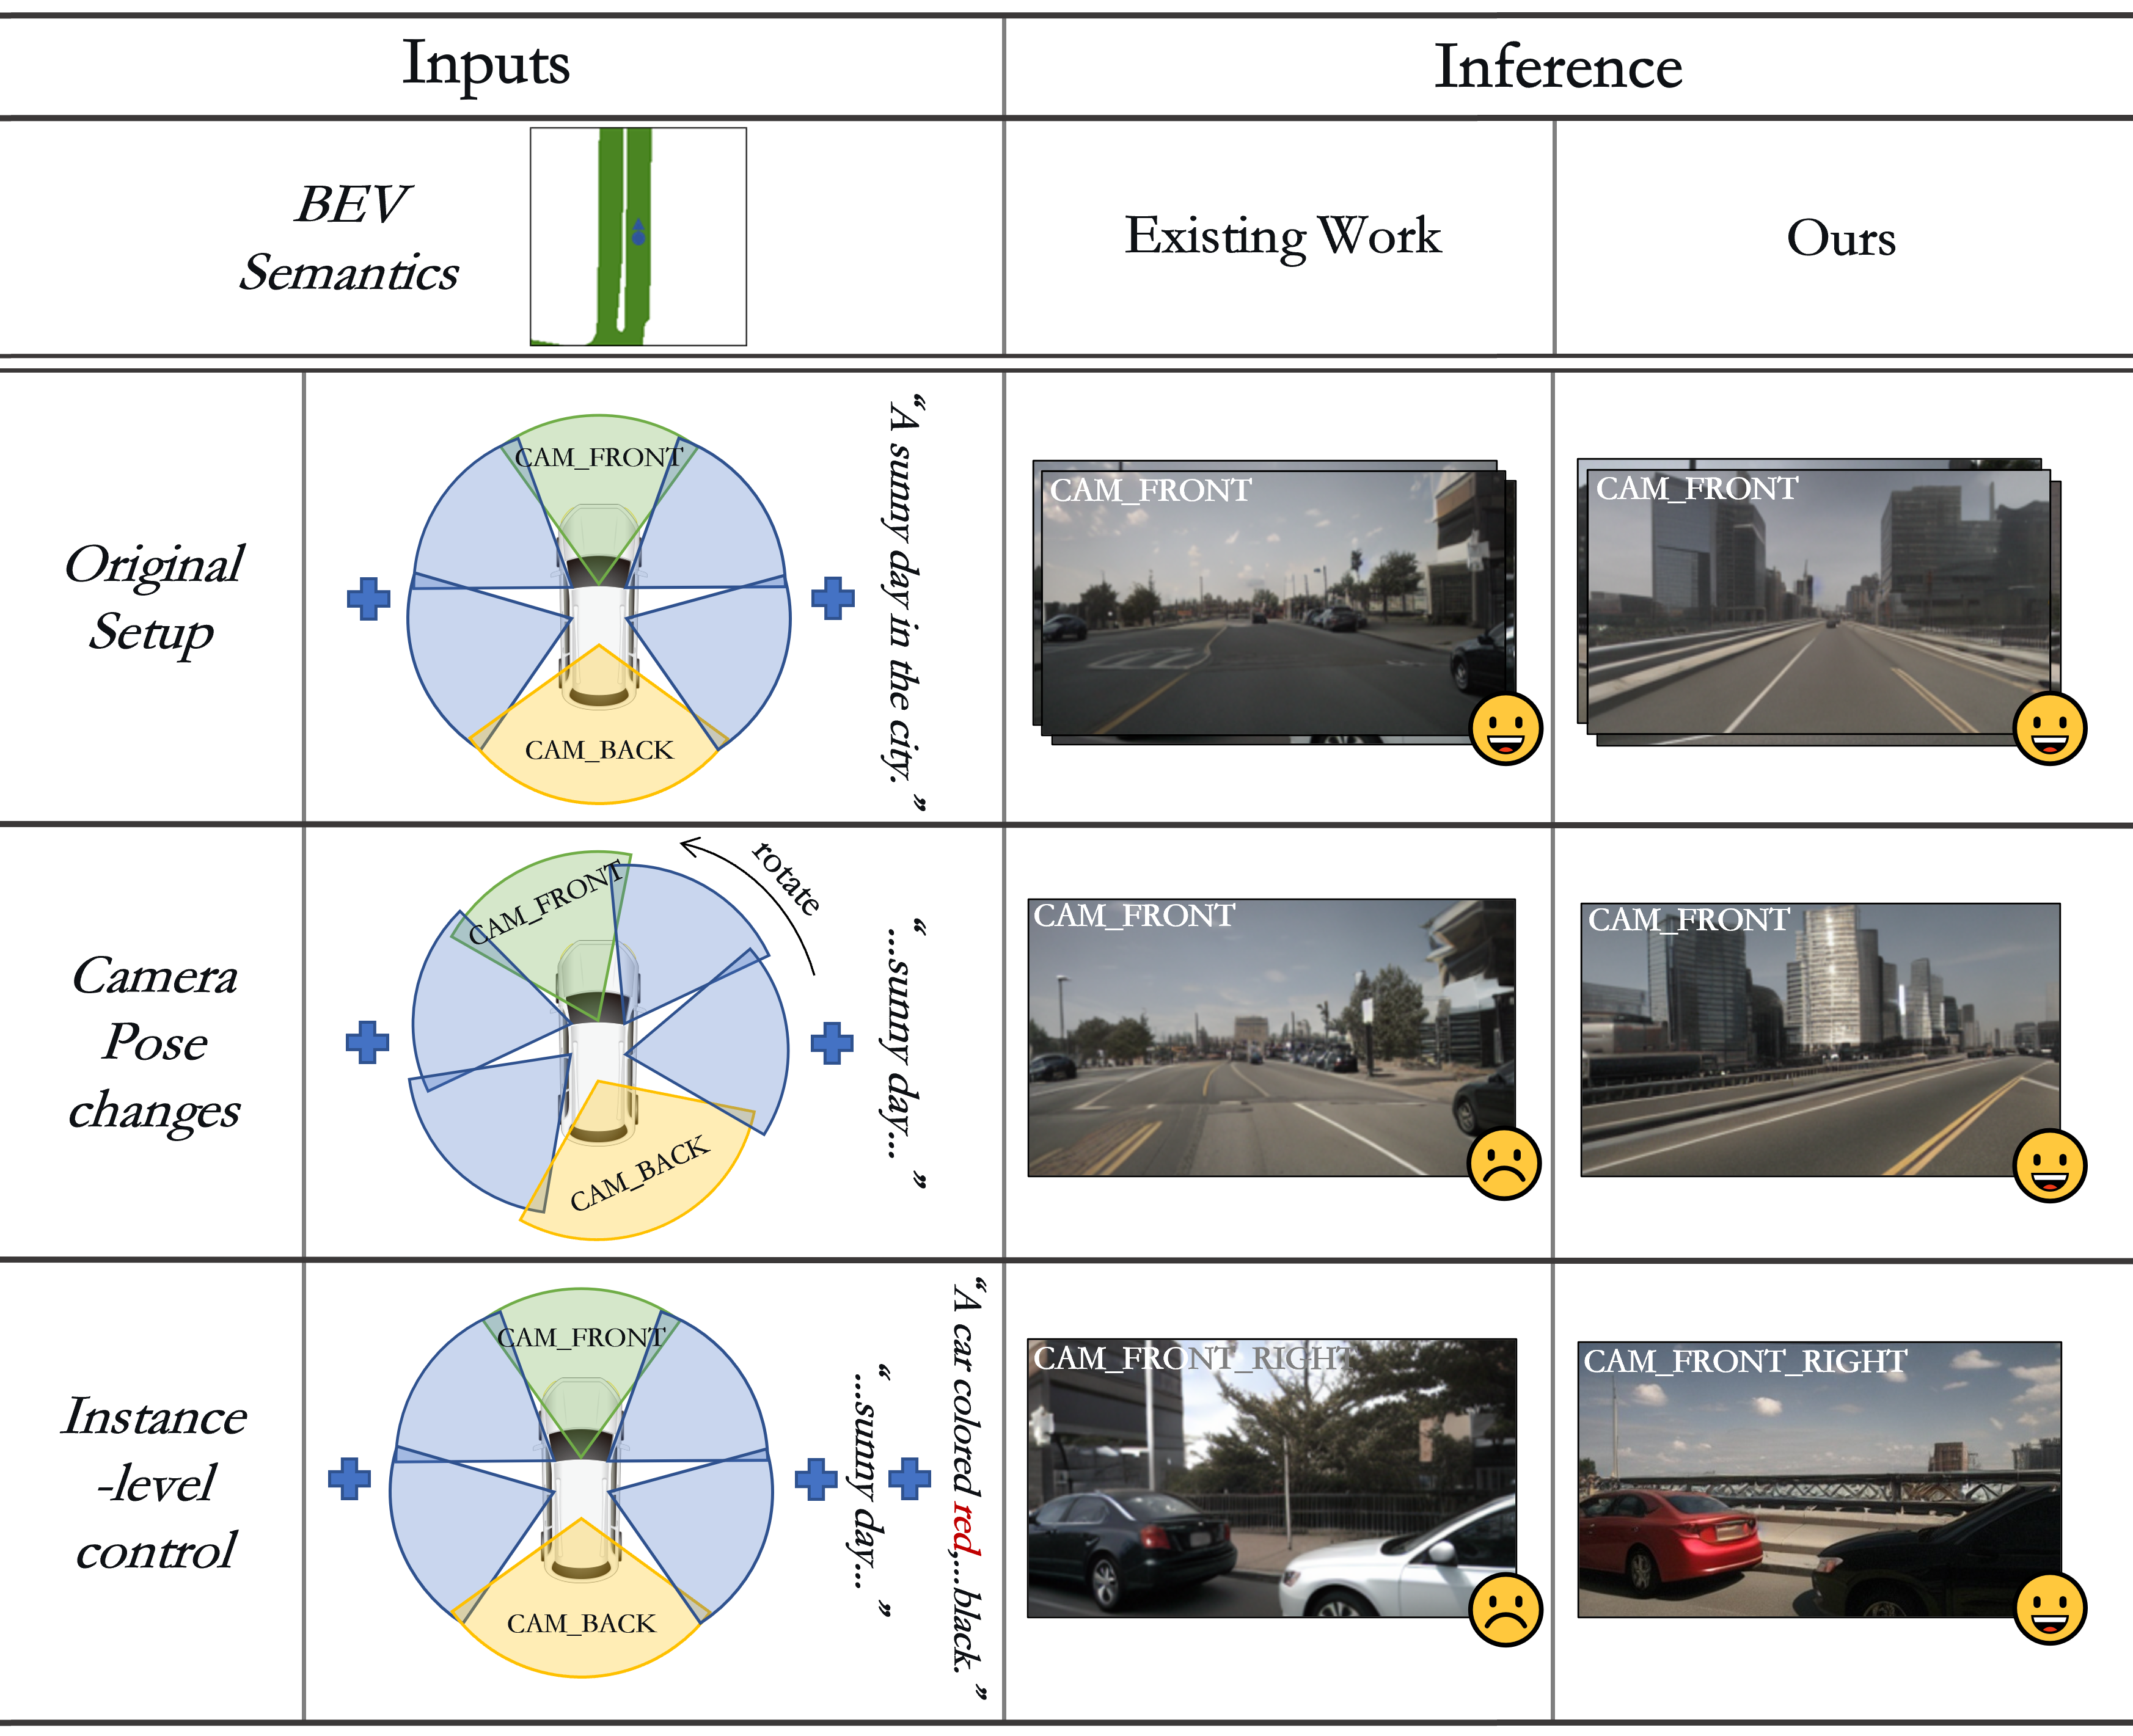
\includegraphics[width=0.9\linewidth]{figures/teaser.png}
\caption{Our MVPbev is able to generate multi-view perspective images with BEV semantics and text prompts. More importantly, MVPbev allows test-time view-point and instance-level control, significantly improving its generalizability. % of existing work.
}
\label{fig:teaser}
\end{figure}
% Thanks to our special initialization and de-nosing processes that explicitly leverage local consistency in latents, MVPbev is able to process perspective semantics in parallel with a pre-trained text-to-image diffusion model and produces multi-view perspective images. Our extensive experiments on NuScenes demonstrate that our method is capable of generating high-resolution photorealistic images from text descriptions with thousands of training samples, surpassing the state-of-the-art methods under various evaluation metrics. We further demonstrate the advances of our method under comprehensive human analysis. Our code and model will be made available.

% or neglect layout consistency, our method MVPbev simultaneously generates images of different perspective views with cross-view awareness, effectively enforcing consistency both visually and semantically. Specifically, our method firstly projects given BEV semantics to perspective view with given camera parameters, which explicitly leverages global semantic coherency. Then we introduce a multi-view attention module to implicitly enforce global consistency among overlapping views w.r.t. cross-view homography. Thanks to our special initialization and de-nosing processes that explicitly leverage local consistency in latents, MVPbev is able to process perspective semantics in parallel with a pre-trained text-to-image diffusion model and produces multi-view perspective images. Our extensive experiments on NuScenes demonstrate that our method is capable of generating high-resolution photorealistic images from text descriptions with thousands of training samples, surpassing the state-of-the-art methods under various evaluation metrics. For instance, our method outperforms ground truth by $4.53$ in terms of PSNR.  We further demonstrate the advances of our method under comprehensive human analysis. Our code and model will be made available.
\end{abstract}



%Then multi-view perspective semantics are stitched together w.r.t. planer assumption to facilitate interactions between various views. Finally, our method processes stitched perspective semantics in parallel with a pre-trained text-to-image diffusion model, while integrating novel homographical loss to enforce global visual consistency. 

%%
%% The code below is generated by the tool at http://dl.acm.org/ccs.cfm.
%% Please copy and paste the code instead of the example below.
%%
%%
%% The code below is generated by the tool at http://dl.acm.org/ccs.cfm.
%% Please copy and paste the code instead of the example below.
%%
\begin{CCSXML}
<ccs2012>
   <concept>
       <concept_id>10010147.10010178.10010224.10010225.10010227</concept_id>
       <concept_desc>Computing methodologies~Scene understanding</concept_desc>
       <concept_significance>300</concept_significance>
       </concept>
   <concept>
       <concept_id>10010147.10010178.10010224.10010225</concept_id>
       <concept_desc>Computing methodologies~Computer vision tasks</concept_desc>
       <concept_significance>500</concept_significance>
       </concept>
 </ccs2012>
\end{CCSXML}

\ccsdesc[300]{Computing methodologies~Scene understanding}
\ccsdesc[500]{Computing methodologies~Computer vision tasks}
%%
%% Keywords. The author(s) should pick words that accurately describe
%% the work being presented. Separate the keywords with commas.
\keywords{Test-time controllability, cross-view consistency, image generation}

%% A "teaser" image appears between the author and affiliation
%% information and the body of the document, and typically spans the
%% page.
% \begin{teaserfigure}
%   \includegraphics[width=\textwidth]{sampleteaser}
%   \caption{Seattle Mariners at Spring Training, 2010.}
%   \Description{Enjoying the baseball game from the third-base
%   seats. Ichiro Suzuki preparing to bat.}
%   \label{fig:teaser}
% \end{teaserfigure}

% \received{20 February 2007}
% \received[revised]{12 March 2009}
% \received[accepted]{5 June 2009}

%%
%% This command processes the author and affiliation and title
%% information and builds the first part of the formatted document.
\maketitle

\section{Introduction}
\label{sec:intro}
Multi-view perspective images are beneficial for autonomous driving tasks~\cite{caesar2020nuscenes}. Nowadays, multi-view cameras, including ones mounted in the front and on the side, have become basic requirements in large driving datasets, such as NuScenes~\cite{caesar2020nuscenes}, Argoverse~\cite{chang2019argoverse} and Waymo~\cite{sun2020scalability}. Typically, images from multiple cameras’ views are perceived and further represented in Bird-Eye-View(BEV)~\cite{Wang_2019_CVPR}, where downstream tasks such as prediction and planning take place later on~\cite{Narayanan_2021_CVPR,Dauner2023CORL}. Intuitively, the BEV allows more interpretability as it provides a tangible interface to the real world, thus is beneficial and practical for higher-level modeling and decision making~\cite{Liu_2020_CVPR,Liu_2022_CVPR}. 

Though being of great importance in autonomous driving tasks, reliable BEV representation requires a large amount of data during the training stage, which can be time-consuming to obtain or annotate. One intuitive solution to this data issue is to obtain diverse perspective RGB images as well as their corresponding BEV semantics with generative models. 
% To this end, the simulation has been an effective method to address this data issue. 
Diverse yet plausible BEV semantics, compared to their corresponding perspective RGB or semantics, are much easier to simulate in a realistic manner with the help of parametric representations~\cite{Wang_2019_CVPR}. To this end, it is natural and practical to assume that BEV semantics, rather than perspective RGB images, are given.
%a natural to resolve this problem is to generate perspective RGB with given BEV semantics. Then 
Then the remaining question is to generate cross-view visually and semantically consistent photorealistic RGB images with known BEV semantics.

Despite the progress of generative models with constraints~\cite{zhang2023adding}, there are three main drawbacks in existing attempts to address this cross-view image generation problem~\cite{Tang2023mvdiffusion,gao2023magicdrive,swerdlow2023street}. Firstly, existing frameworks rely heavily on the training samples, leading to unsatisfactory test-time controllability. For instance, changing camera poses or providing extra control on object instance is beyond prior art. Moreover, cross-view consistency is not well enforced, resulting in inconsistent visual effects in overlapping FOVs. Finally, no thorough human analysis is performed on image generation tasks, resulting in un-interpretable comparison results.

% First of all, existing methods suffer from dramatic changes in viewpoints, making it impossible to generate perspective images with control signals in BEV. Secondly, consistency is not well enforced in overlapping FOVs, leading to unsatisfactory and inconsistent visual results. Finally, no thorough human analysis is performed on image generation tasks, resulting in un-interpretable comparison results.

% Firstly, though providing quite consistent background stuff with noticeable interactions, controllability is lacking in autoregressive-based methods~\cite{??}. In the meantime, foreground objects are also handled poorly, reflecting the fact that delicate interactions are missing in this line of work. More recent work~\cite{??} aims to provide more control with the help of diffusion models~\cite{??}. However, it suffers from image inconsistency, especially for background contents at overlapping field-of-view (FoV) of multiple cameras. 

To this end, we propose a novel two-stage method MVPbev that aims to generate controllable multi-view perspective RGB images with given BEV semantics and text prompts by explicitly enforcing cross-view consistency (See Fig.~\ref{fig:teaser}). Unlike existing work that lacks the test-time generalizability, MVPbev further allows both view-point and detailed text prompt changes at test-time, providing satisfactory performances under human analysis without requiring additional training data. To achieve that, MVPbev consists of two stages, or view projection and scene generation stages. The former stage transforms the given BEV semantics to multiple perspective view w.r.t. camera parameters. On the one hand, it enforces global consistency across views with explicit geometric transformation. On the other hand, such a design decouples the two stages, allowing the second stage to better capture view-point-invariant properties. The second stage of MVPbev starts from a pre-trained stable diffusion (SD) model. By explicitly incorporating a cross-view consistent module, together with our noise initialization and de-noising processes design, it can produce multi-view visually consistent and photo-realistic images, especially at overlapping FOVs. To further improve the test-time generalizability on objects, our MVPbev handles foreground instances and background layout individually, leading to better controllability during inference.
% The former focuses on not only the visual styling of RGB images from multiple cameras but also the overall semantic layout consistency w.r.t. both BEV semantics and text prompts. The latter, on the other hand, considers contents at overlapping FOVs of multiple cameras. Specifically, the global semantic layout consistency is firstly achieved with strict geometry by projecting the BEV semantics to multiple perspective views with given camera parameters. Meanwhile, the global and local visual consistencies are leveraged with the help of our multi-view attention module, as well as the noise initialization and de-noising processes. 
%our image stitching module, where dataset-wise camera homography is estimated in training RGB images and then used to stitch perspective semantics when overlapped FOV happens. 
% Compared to existing work, our multi-view attention module implicitly models the interactions between overlapping views, leading to more consistent prediction at overlapping areas. Finally, our MVPbev processes perspective semantics in parallel with a pre-trained text-to-image diffusion model, leveraging special designs of initialization and de-noising to enforce local visual consistency explicitly. 

We validate our ideas on NuScenes~\cite{caesar2020nuscenes} and follow the standard split. In contrast to methods that focus on improvements over downstream tasks or semantic consistency, we include additional extensive human analysis, especially on visual consistency over overlapping FOVs, across multiple views, and test-time view point and text prompt changes. We demonstrate that our proposed method not only provides better test-time controllability and generalizability, but also gives high-quality cross-view RGB images.
% more cross-view consistent RGB both visually and semantically.
In short, our contribution can be summarized as follows:
\begin{itemize}
    \item A novel multi-view image generation method that is capable of producing semantically and visually consistent perspective RGB images from BEV semantics, with only thousands of images as training data.
    \item A more controllable yet extendable algorithm that gives realistic perspective RGB images.
    \item State-of-the-art performances on large driving datasets, with comprehensive human analysis\footnote{Our code, data and model can be found in \url{https://github.com/kkaiwwana/MVPbev}.}.
\end{itemize}
% \begin{packed_lefty_item}
% \item A novel multi-view image generation method that is capable of producing semantically and visually consistent perspective RGB images from BEV semantics, with only thousands of images as training data.

% \item A more controllable yet extendable algorithm that gives realistic perspective RGB images.

% \item State-of-the-art performances on large driving datasets, with comprehensive human analysis.

% \item We extend the existing NuScenes dataset with language descriptions for background.
% \end{packed_lefty_item}

\section{Related Work}
\label{sec:relatedwork}

\begin{figure*}[t]
\centering
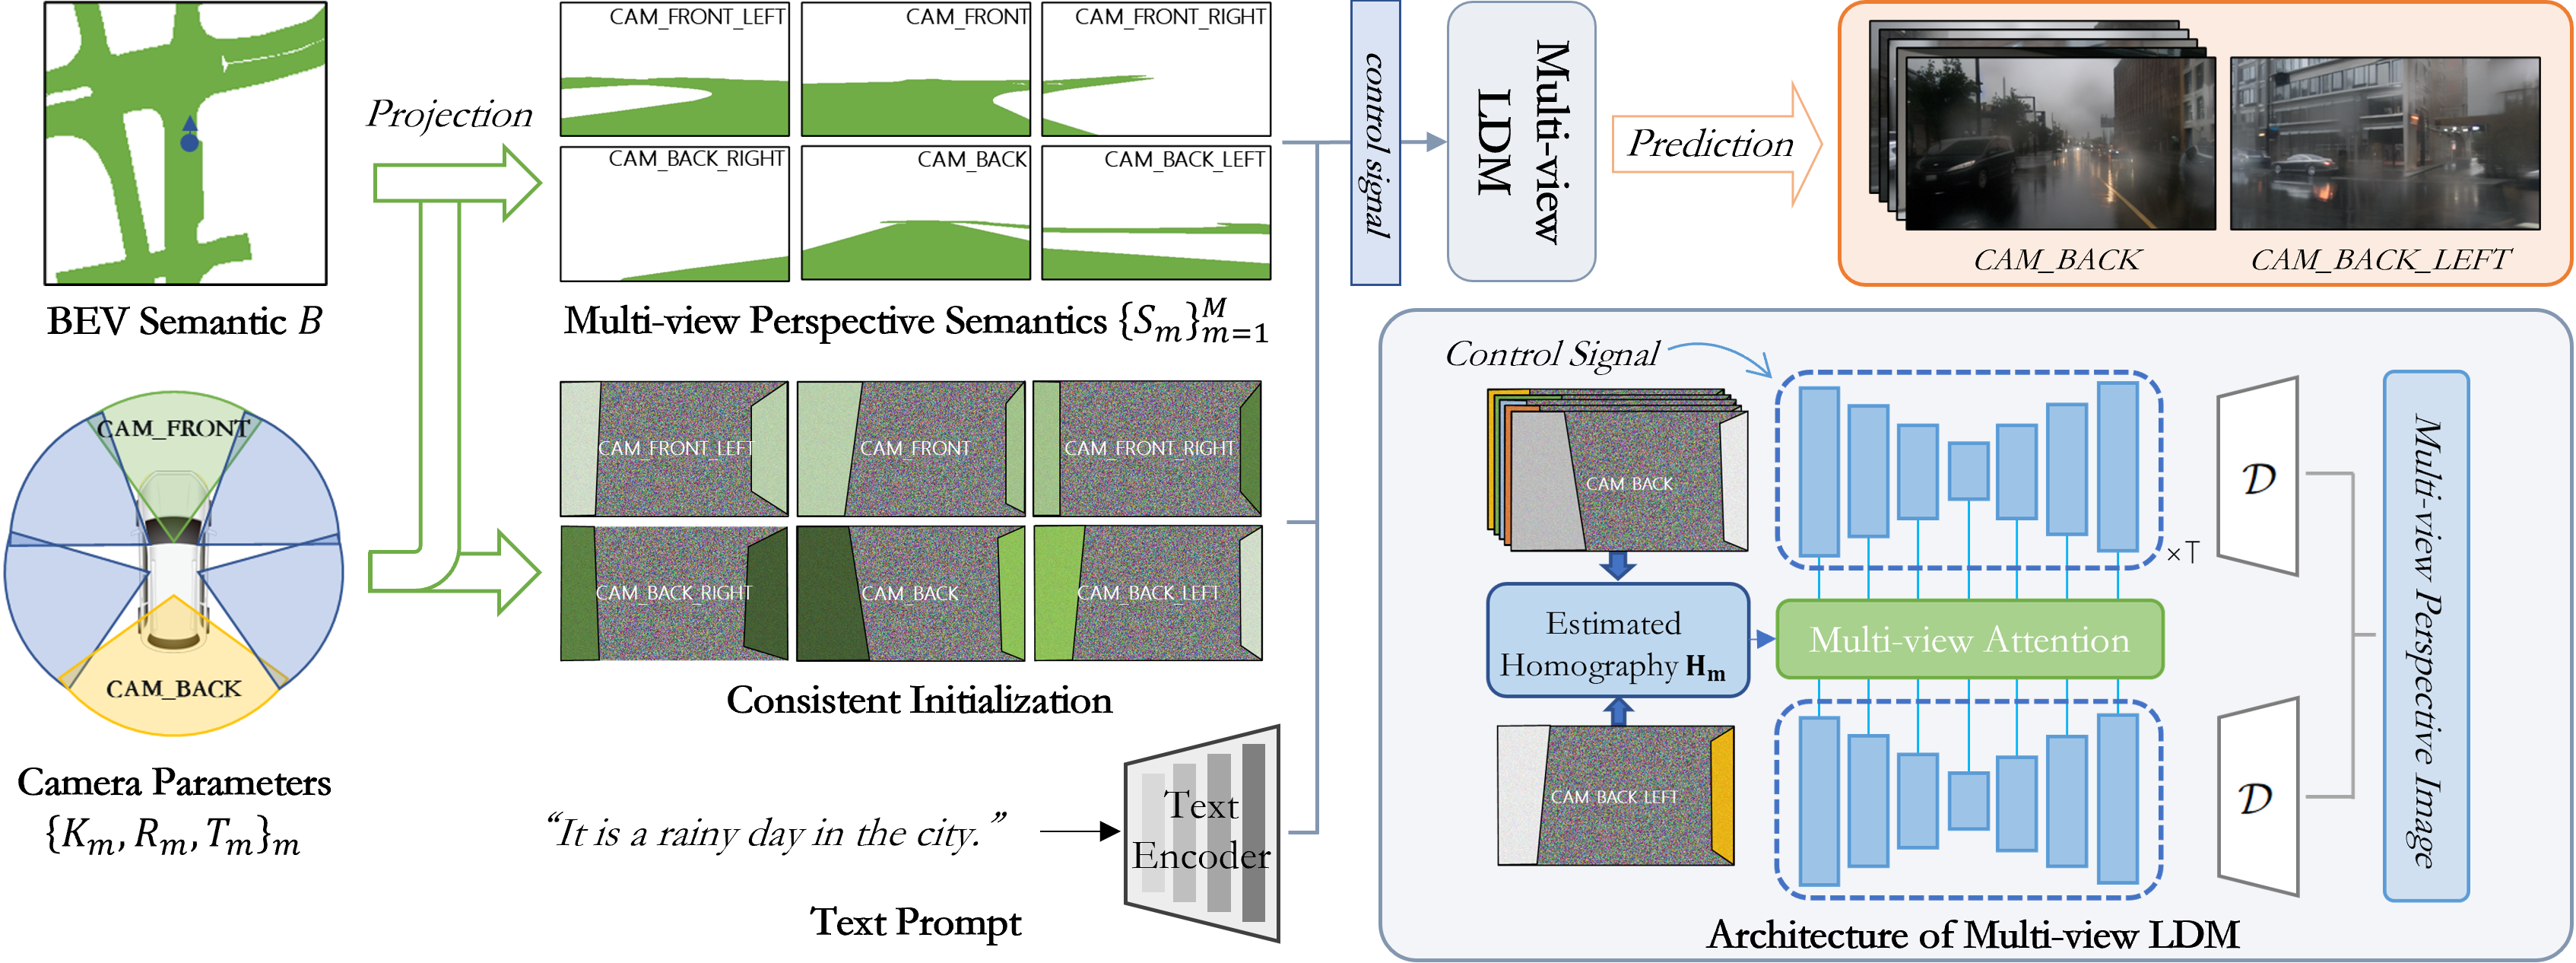
\includegraphics[width=0.95\linewidth]{figures/main.png}
\caption{MVPbev consists of two stages. The first stage projects BEV semantics to perspective view with camera parameters to maintain global semantic consistency. The second stage parses both perspective semantics and text prompts, and generates multi-view images with both visual consistency and test-time instance-level control by explicit enforcing in latent.
}
\label{fig:main}
\end{figure*}

Image editing~\cite{imageedit} and generation~\cite{rombach2021highresolution} are heated topics in computer vision. Though this can be related to a vast literature, we would focus on two lines of work, conditional image generation and novel view image synthesis, as they are closely relevant.

\noindent{\textbf{Conditional image generation}} Generative models, e.g., Gaussian Mixture model~\cite{rasmussen1999infinite} and Bayesian network~\cite{Jensen2001Bayesian}, have been a long-term research problem in machine learning and computer vision as it is able to explain complex data distribution. In particular, generative models of images are not only of great importance for unsupervised feature learning, but also enable applications such as image editing~\cite{imageedit,kawar2023imagic}. With the rise of deep learning techniques, such as auto-regressive models~\cite{chan2005probabilistic}, variational autoencoders (VAEs)~\cite{kingma2013auto}, and generative adversarial networks (GANs)~\cite{goodfellow2020generative}, as well as the emerging of huge amount of data~\cite{imagenet}, we observe photorealistic images with very good quality. Among them, conditional GANs have been well explored where various constraints, including discrete labels, text, and images, are considered. More recently, stable diffusion models~\cite{rombach2021highresolution} are widely used to generate detailed images conditioned on text descriptions. Compared to the prior art, they not only demonstrate SOTA image generation quality, but also showcase great generalizability with the help of foundation models~\cite{li2023blip}. Later on, Controlnet~\cite{zhang2023adding} largely improves the overall performance of diffusion models without losing the original robustness by allowing a diverse set of conditional controls, e.g., depth, semantics, or sketches. Despite impressive progress, multi-view or cross-view text-to-image generation still confronts issues of computational efficiency and consistency across views. To this end, MVDiffusion~\cite{Tang2023mvdiffusion} proposes a novel correspondence-aware attention module to create multi-view images from text with the ability to maintain global correspondence. Though providing good multi-view RGB images, MVDiffusion fails to generalize to more dramatic viewpoint changes or smaller overlapping areas. Perhaps the co-current work, including BEVGen~\cite{swerdlow2023street}, BEVControl~\cite{yang2023bevcontrol}, and MagicDrive~\cite{gao2023magicdrive},  are the closest to ours. The first one generates multi-view visual consistent images based on the BEV semantics by employing an auto-regressive transformer with cross-view attention. While the last two work with image sketches/semantics and text, and utilizes cross-view cross-object attention to focus more on consistency on individual contents. However, none of existing work allows test-time generalizability, e.g., view-point changes or detailed instance-level text prompts. Nor do they conduct human analysis on image generation quality. In contrast, we propose to exploit both global and local consistency to leverage semantic and visual coherency, together with our training-free objects control method to enforce detailed instance-level control. Moreover, we provide comprehensive human analysis to demonstrate the effectiveness of our method in a more reliable manner. 

% detailed human analysis are missing. In this work, we propose to exploit both global and local consistency to leverage semantic and visual coherency. In the meantime, we extend NuScenes with text prompts and conduct comprehensive human analysis to demonstrate the effectiveness of our method. 
%Perhaps the co-current work, specifically the BEVGen~\cite{?} and BEVControl~\cite{?}, are the closest to ours. The former generates multi-view visual consistent images based on the BEV semantics by employing an auto-regressive transformer with cross-view attention. In contrast, the latter works with image sketches and text, and utilizes cross-view cross-object attention to focus more on consistency on individual contents. 
% Though providing good multi-view RGB images, there are two main drawbacks of the above-mentioned methods. Firstly, they fail to enforce the visual consistency at overlapping FOVs, especially for the background. Secondly, an evaluation of the method's robustness and
% detailed human analysis are missing. In this work, we propose to exploit both global and local consistency to leverage semantic and visual coherency. In the meantime, we extend NuScenes with text prompts and conduct comprehensive human analysis to demonstrate the effectiveness of our method. 

\noindent{\textbf{Novel view image synthesis}} There are two broad categories in which the novel view synthesis methods can be divided into geometry-based and learning-based approaches. The former tries to first estimate (or fake) the approximate underlying 3D structures, followed by applying some transformation to the pixels in the input image to produce the output~\cite{avidan1997novel,zhou2016view}. The latter, on the other hand, argues that novel view synthesis is fundamentally a learning problem, because otherwise it is woefully under-constrained. More recently, neural radiance fields (NeRF)~\cite{mildenhall2021nerf}, which belong to the second category, have shown impressive performance on novel view synthesis of a specific scene by implicitly encoding volumetric density and color through a neural network. Starting from small-scales~\cite{mildenhall2021nerf}, scene-level NeRFs, such as Block-NeRF~\cite{tancik2022block}, are also proposed such that important use-cases, e.g., autonomous driving~\cite{caesar2020nuscenes} and aerial surveying~\cite{kaiser2017learning} are enabled by reconstructing large-scale environments. In contrast, our method takes the input as BEV semantics and text description and outputs multi-view perspective RGB. 
%, allowing more generalizability over modality and view-point changes. % and fine-grained control.
% Our method not only allows more controllability, but also enforces cross-view consistency both visually and semantically.
\section{Our Method}
\label{sec:method}

\begin{figure}[b!]
\centering
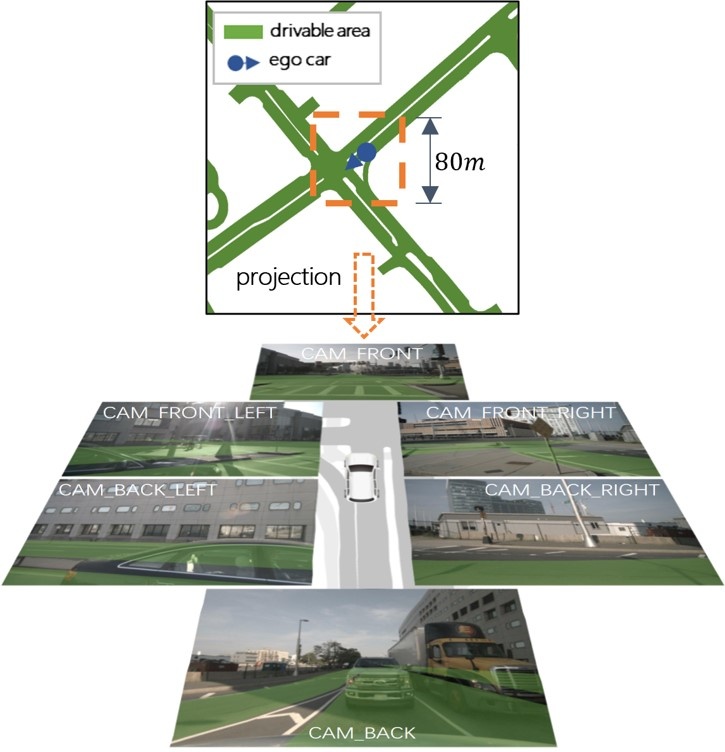
\includegraphics[width=0.9\linewidth]{figures/bev_projection.jpg}
\caption{We visualize our BEV project process. Given a BEV semantic map $\textit{B}$, we project it to multiple perspective views. We overlay the semantics on the original RGB images in perspective view for better comparison.  
}
\label{fig:bev_proj}
\end{figure}

Our method aims to generate multi-view perspective images from text prompts given pixel-level BEV semantic correspondences. Specifically, we denote the BEV semantics as $\textit{B}\in\mathbb{R}^{H_b\times W_b\times c_b}$, with the ego car assumed to be located at the center. And $H_b$, $W_b$, and $c_b$ are the height, width, and number of semantic classes of $\textit{B}$, respectively. Our goal is to generate a set of perspective RGB images with resolution $H$ by $W$, or $\{I_m\}_m$ in particular, under $M$ virtual camera views. And the $m$-th perspective image is referred to as $I_m\in\mathbb{R}^{H\times W\times 3}$ where $m=\{1,\dots,M\}$. In particular, we assume the intrinsics, extrinsic rotation, and translation of the $m$-th camera are given and denote them as $K_m$, $R_m$, and $T_m$, respectively. 

As described above, we obtain visually coherent multi-view images by leveraging both global and local consistency in implicit and explicit manners. Specifically, our method consists of two stages. Our first stage takes BEV semantics $\textit{B}$ as well as $\{K_m,R_m,T_m\}_m$ as input and projects BEV semantics to each perspective view w.r.t. its camera parameter set, denoting as $S_m\in\mathbb{R}^{H\times W\times c_b}$ for the $m$-th view. The second stage parses $\{S_m\}_{m=1}^M$ and text prompts as input. And it produces RGB images from $M$ perspective views. $I_m$ denotes the generated RGB image from $m$-th view. 
% Thanks to the multi-view consistency module, our second stage is capable of implicitly leveraging global visual consistency among overlapping views when producing $M$ perspective RGB images according to perspective semantics and text prompts. 
%or $\{I_m\}_{m=1}^M.$ 
%Then the perspective semantics are stitched together according to the homography between overlapping camera views, leading to $\hat{S}_m\in\mathbb{R}^{\hat{H}\times\hat{W}\times c_b}$. 
More specifically, our first projection stage enforces global semantic consistency between BEV and perspective view explicitly with the help of geometric transformation. Meanwhile, the generation stage imposes consistency implicitly among overlapping perspective views with a multi-view attention module. Finally, we propose to explicitly enforce the visual cues at overlapping FOVs to be coherent with our novel training initialization and de-noising designs. The overall pipeline of MVPbev can be found in Fig.~\ref{fig:main}. We provide more details of the first and second stages in Sec.~\ref{sec:pers_map} and Sec.~\ref{sec:model} respectively. And the model training process is described in Sec.~\ref{sec:model_train}.

%The second stage of our method then parses the generated semantics $\hat{S}_m$ and text prompt, and produces multi-view images $\{I_m\}_m$. Specifically, we would highlight our homographic transformation module, which aims to enforce homographic constraints across multi-view feature maps. Details of the second step can be found in Sec.~\ref{sec:model}.

% We introduce the first step which aims to enforce cross-view consistency by generating corresponding semantics in Sec.~\ref{sec:pers_map}. Later on, our second step receives the generated semantics as well as paired text description, and produces multi-view consistent images. Details of the second step can be found in Sec.~\ref{sec:model}.

\subsection{Semantic-consistent view projection}\label{sec:pers_map}
Assuming that diverse yet plausible BEV semantics $\textit{B}$ can be obtained effortlessly with existing simulation methods~\cite{Wang_2019_CVPR}, the first fundamental problem that our method should address is to maintain cross-view semantic consistency from $\textit{B}$ to perspective images $\{I_m\}_m$. Secondly, contents at overlapping FOVs should also be coherent. For example, not only the background classes, such as buildings or trees, but also the foreground road participants, should be of similar appearance when they appear in different views. To this end, we first propose to project BEV semantics to $M$ perspectives view with camera parameters, which generates $\{S_m\}_{m=1}^M$ perspective semantics. Compared to existing work~\cite{zhang2023adding}, our projection step ensures semantic-wise consistency between BEV and perspective views with the help of geometry constraints, leading to fewer accumulative errors at the generation step (See examples in Fig.~\ref{fig:bev_proj}). % And our projection results can be found in Fig.~\ref{fig:bev_proj}.  

\subsection{View consistent image generation}\label{sec:model}
%Though being well-motivated and proved to be effective in terms of handling foreground objects~\cite{??}, 
Simply working on individual perspective semantics may lead to inconsistent content across different views, especially at overlapping FOVs. For instance, the buildings and the vegetation that appear at the FOVs among multiple views, e.g., the front, front-right, back, and back-left, have different appearances. This is due to the lack of interactions among cross-view cameras. We would like to note that such inconsistency would be reflected by neither BEV layout segmentation nor object detection metrics as it has influences on background classes only. 

Motivated by this, we propose to focus on these overlapping areas both methodologically and experimentally. As for our method, we apply strong coherency constraints on the background content by estimating the homography of overlapping areas, followed by a multi-view attention module to implicitly enforce the styles at various views to be coherent w.r.t. estimated corresponding points. 
% Moreover, we introduce novel initialization and de-noising processes to explicitly enforce latent features at overlapping areas to be consistent. 
%Later on, our generation stage works on the stitched images rather than the individual ones (See Sec.~\ref{sec:model} for more details). 
In this case, appearance consistency can be enforced not only on the background layout areas where the semantics are provided, but also on the other regions where control signals are missing. 
As for the evaluation purpose, we introduce human analysis to provide reliable evaluations on whether the generated images, especially the overlapping regions, are realistic or not. We demonstrate that our proposed method copes with background consistency well (See Sec.\ref{sec:experiment} for quantitative and qualitative results).

% \noindent{\textbf{Homography estimation}} 
\noindent{\textbf{Homography estimation}} We take the initial step towards enforcing visual consistency at overlapping FOVs by estimating the overlapping regions. To this end, we propose to compute the homography between images with overlapping FOVs. As illustrated in many driving datasets, one view generally overlaps with views on its left and right sides. Therefore, for the $m$-th view, we only need to consider $m_l=\mod(m+M-2,M)+1$ and $m_r=\mod(m+1,M)$, which are the left and right views of the $m$-th view respectively. Then we estimate the homography from view $m_r$ to view $m$ and denote the mapping function as $H_m$. Consequently, the $p=[x,y]$ coordinate in the $m$-th view will be mapped to coordinate $\hat{p}=[\hat{x},\hat{y}]$ in view $m_r$. Or $\hat{p}=H_m(p)$. Similarly, we define an inverse mapping $\overline{H}_m$ that maps $\hat{p}$ in $I_{m_r}$ to $p$ in $I_{m}$. 

%Denoting the left and right views of the $m$-th view as $m_l=\mod(m+M-2,M)+1$ and $m_r=\mod(m+1,M)$ respectively, 

% We provide one set of examples of our estimated homography in \textcolor{red}{Fig.~\ref{??}}. As can be found in this figure, our estimated homography is of high quality as we are able to generate reasonable results when stitching images with it. 

\begin{figure}[ht]
\centering
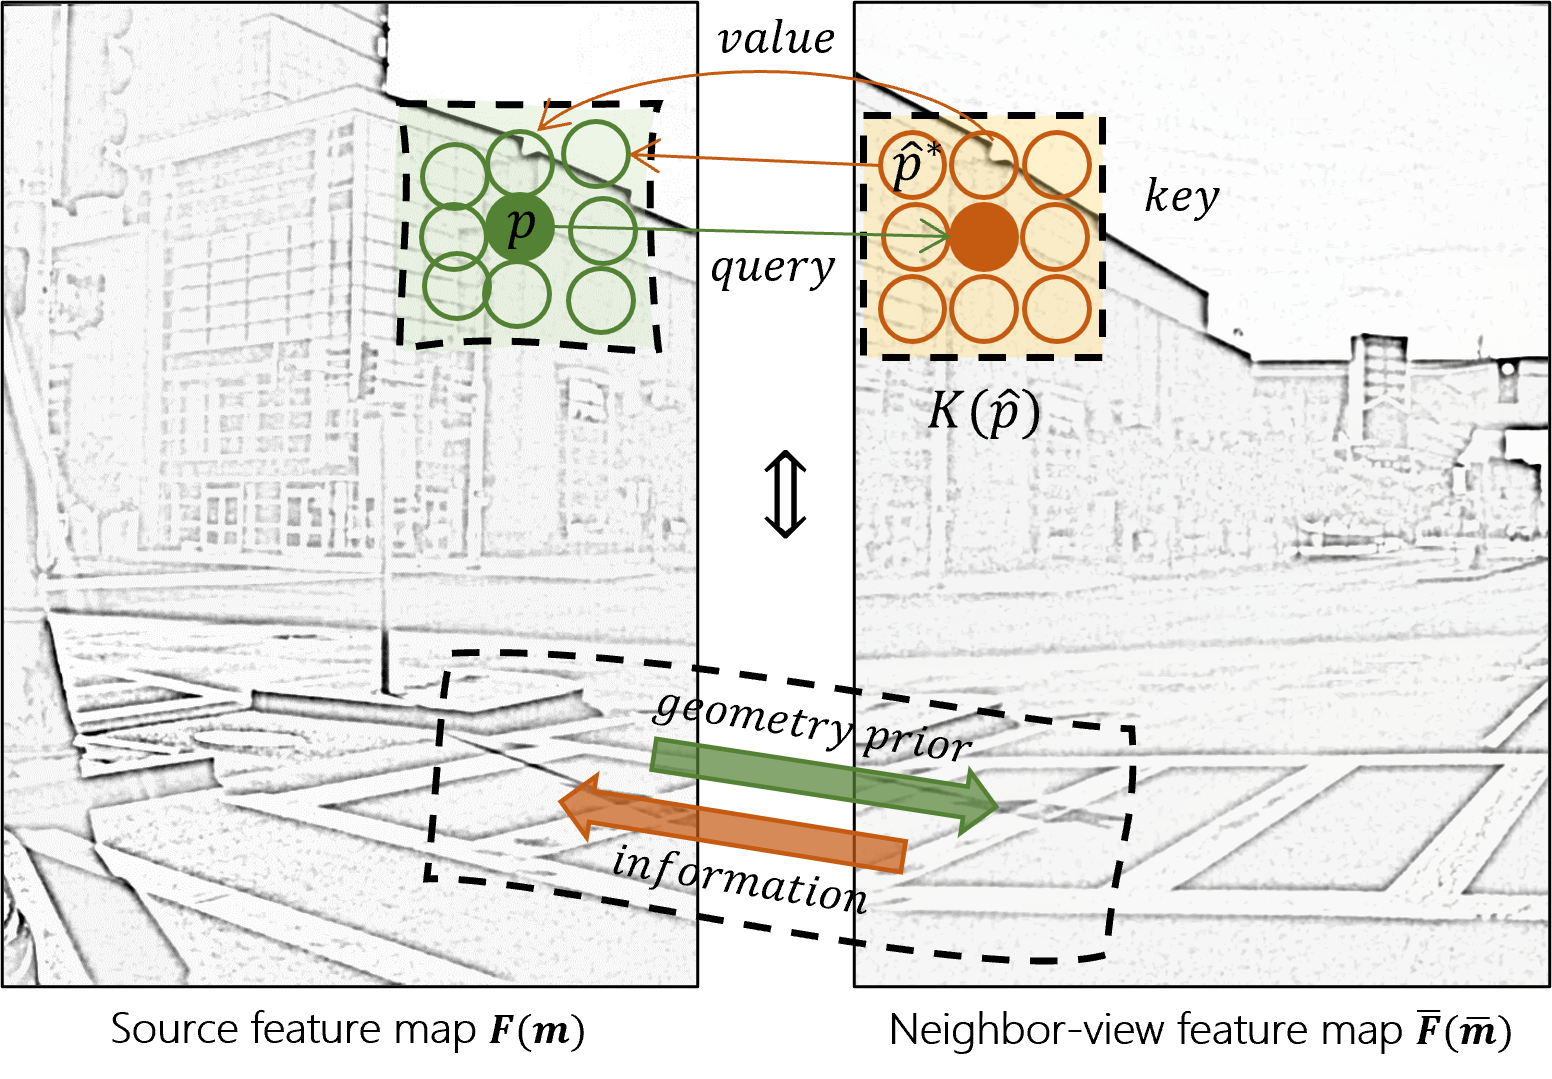
\includegraphics[width=0.9\linewidth]{figures/cross_view_attention.png}
\caption{Our multi-view attention module implicitly exploits the cross-view consistency by aggregating information from the target feature pixels in neighbour views.
% w.r.t. estimated homography. 
%Specifically, it aggregates information from the target feature pixels in neighbour views, which are obtained by homographic transformation, to the source.
}
\label{fig:cross_view}
\end{figure}

% \noindent{\textbf{Multi-view attention module}} 
\noindent{\textbf{Multi-view attention module}} What makes a set of views unrealistic? The first and foremost thing is the incoherence among images. In other words, realistic ones must appear consistent, as if they were taken in the same physical location at the same time of a day. More specifically, the visual styling of this set of images needs to be consistent such that all of them appear to be created in the same geographical area (e.g., urban vs. rural), time of day, with the same weather conditions, and so on. To this end, we introduce a multi-view attention module such that when generating the RGB from the $m$-th view, the views on its left and right sides 
% , or view $m_l=\mod(m+M-2,M)+1$ and view $m_r=\mod(m+1,M)$ respectively, 
% ~\footnote{Mathematically, the left and right views of the $m$-th frame should be $\mod(m+M-2,M)+1$ and $\mod(m+1,M)$. We }
are considered. For a token located at position $p$ in the feature
map $F_m$ generated from $m$-th view, we compute the attention output based on the corresponding pixels $K(\hat{p})$ in the feature maps generated by view $\bar{m}\in\{m_r,m_l\}$, where $\hat{p}^*\in K(\hat{p})$ denotes a $K$ by $K$ region centered at $\hat{p}$. Mathematically, we follow a similar formulation as in~\cite{vaswani2017attention} and define our multi-view attention module as:
\begin{equation} 
\mathbf{a}=\sum_{\bar{m}}\sum_{\hat{p}^*}Softmax(\left[Q F_m(p)\right]\cdot\left[K\bar{F}_{\bar{m}}(\hat{p}^*)\right]) V\bar{F}_{\bar{m}}(\hat{p}^*),~\label{equ:global_term}
\end{equation}
where $Q$, $K$, and $V$ are the learnable weights of query, key, and value matrices respectively. $\bar{F}_{\bar{m}}(\hat{p}^*)=F_{\bar{m}}(\hat{p}^*)+d(\overline{H}_m(\hat{p}^*)-p)$. We further denote $d(\cdot)$ as a position encoding to the $F_{\bar{m}}(\hat{p}^*)$ based on the 2D displacement between $p$ and $\overline{H}_m(\hat{p}^*)$. As can be found in Eq.~\ref{equ:global_term}, our multi-view attention module aims to aggregate information from the target feature pixels $K(\hat{p})$ to $p$. We provide a simple illustration of our multi-view attention module in Fig.~\ref{fig:cross_view}.

\subsection{Model training and inference}~\label{sec:model_train}
To train our model, we introduce a multi-view Latent Diffusion Models (LDMs)~\cite{rombach2021highresolution} loss. Basically, the original LDMs consist of a variational autoencoder (VAE) with encoder $\mathcal{E}$ and decoder $\mathcal{D}$, a denoising network $\delta_{\theta}$ and a condition encoder $\tau_{\theta}$. The input image $I_m$ is mapped to a latent space by $\mathbf{l}_m=\varepsilon(I_m)$, where $\mathbf{l}_m\in\mathbb{R}^{h\times w\times c}$. We follow the routine to set $\frac{H}{h}=\frac{W}{w}$ and they both equal to 8. Later on, the latents will be converted back to the image space by $\tilde{I}_m=\mathcal{D}(\mathbf{l}_m)$. The denoising network $\delta_{\theta}$ is a time-conditional UNet, which leverages cross-attention mechanisms to incorporate the condition encoding $\tau_{\theta}(\mathbf{c})$. In our case, $\mathbf{c}$ consists of text-prompt and semantics in perspective view $S_m$. 

\begin{figure}[t]
\centering
\includegraphics[width=0.9\linewidth]{figures/latent_initialization.png}
\caption{We explicitly enforce that the noise value of pixels at overlapping FOV should be consistent across views. 
}
\label{fig:noise_init}
\end{figure}

For each training step, we firstly uniformly sample a shared noise level $t$ from 1 to $T$ for all the multi-view images $\{I_m\}_{m=1}^M$, denoting them as $\{\epsilon^t_m\}_m$. And $\epsilon^t_m\sim\mathcal{N}(0,1)$. To leverage the cross-view consistency, we further enforce these noises to be the same if they correspond to the same pixel. Starting from the first view, or $m=1$, we re-assign value at coordinate $x,y$ of $\epsilon^t_m$, or $\epsilon^t_m(x,y)$, to $\epsilon^t_{m_r}(\hat{x},\hat{y})$. And we repeat the process until $m_r=1$. We provide one example set of our initialized $\{\epsilon^t_m\}_{m=1}^M$ in Fig.~\ref{fig:noise_init}. Finally, our model training objective is defined as:
\begin{equation}
\begin{aligned} 
 \mathcal{L}:=\mathbb{E}_{\{\mathbf{l}_m,\epsilon^t_m\}_{m=1}^M,t,\mathbf{c}}\left[\sum_{m=1}^M\|\epsilon^t_m-\delta_{\theta}^m(\{l_m^t\},t,\tau_{\theta}(\mathbf{c})\|_2^2\right],
 \end{aligned}~\label{equ:loss}
\end{equation}
where $\delta_{\theta}^m$ is the estimated noise for the $m$-th image. And we use $l_m^t$ to denote the noisy latent for the $m$-th image. 

At sampling time, the denoising (reverse) process generates samples in the latent space, and the decoder $\mathcal{D}$ produces RGB images with a single forward pass. To incorporate our idea that pixels at overlapping regions should be visually similar even at different views, we again employ the value assignment process. Similar to the noise initialization step, we re-assign value at coordinate $x,y$ of $l^t_m$, or $l^t_m(x,y)$, to $l^t_{m_r}(\hat{x},\hat{y})$. This re-assignment starts from $m=1$ and does not stop until $m_r$ equals to 1. In experiments, we observe that our design would improve the visual results if applied to up to $\frac{3\times T}{5}$ denoising steps. Otherwise, the performance deteriorates. % More steps would deteriorate the overall performance. 
% We provide some examples in Fig.~\ref{fig:denoise} as a reference. 

% \begin{figure}[ht]
% \centering
% 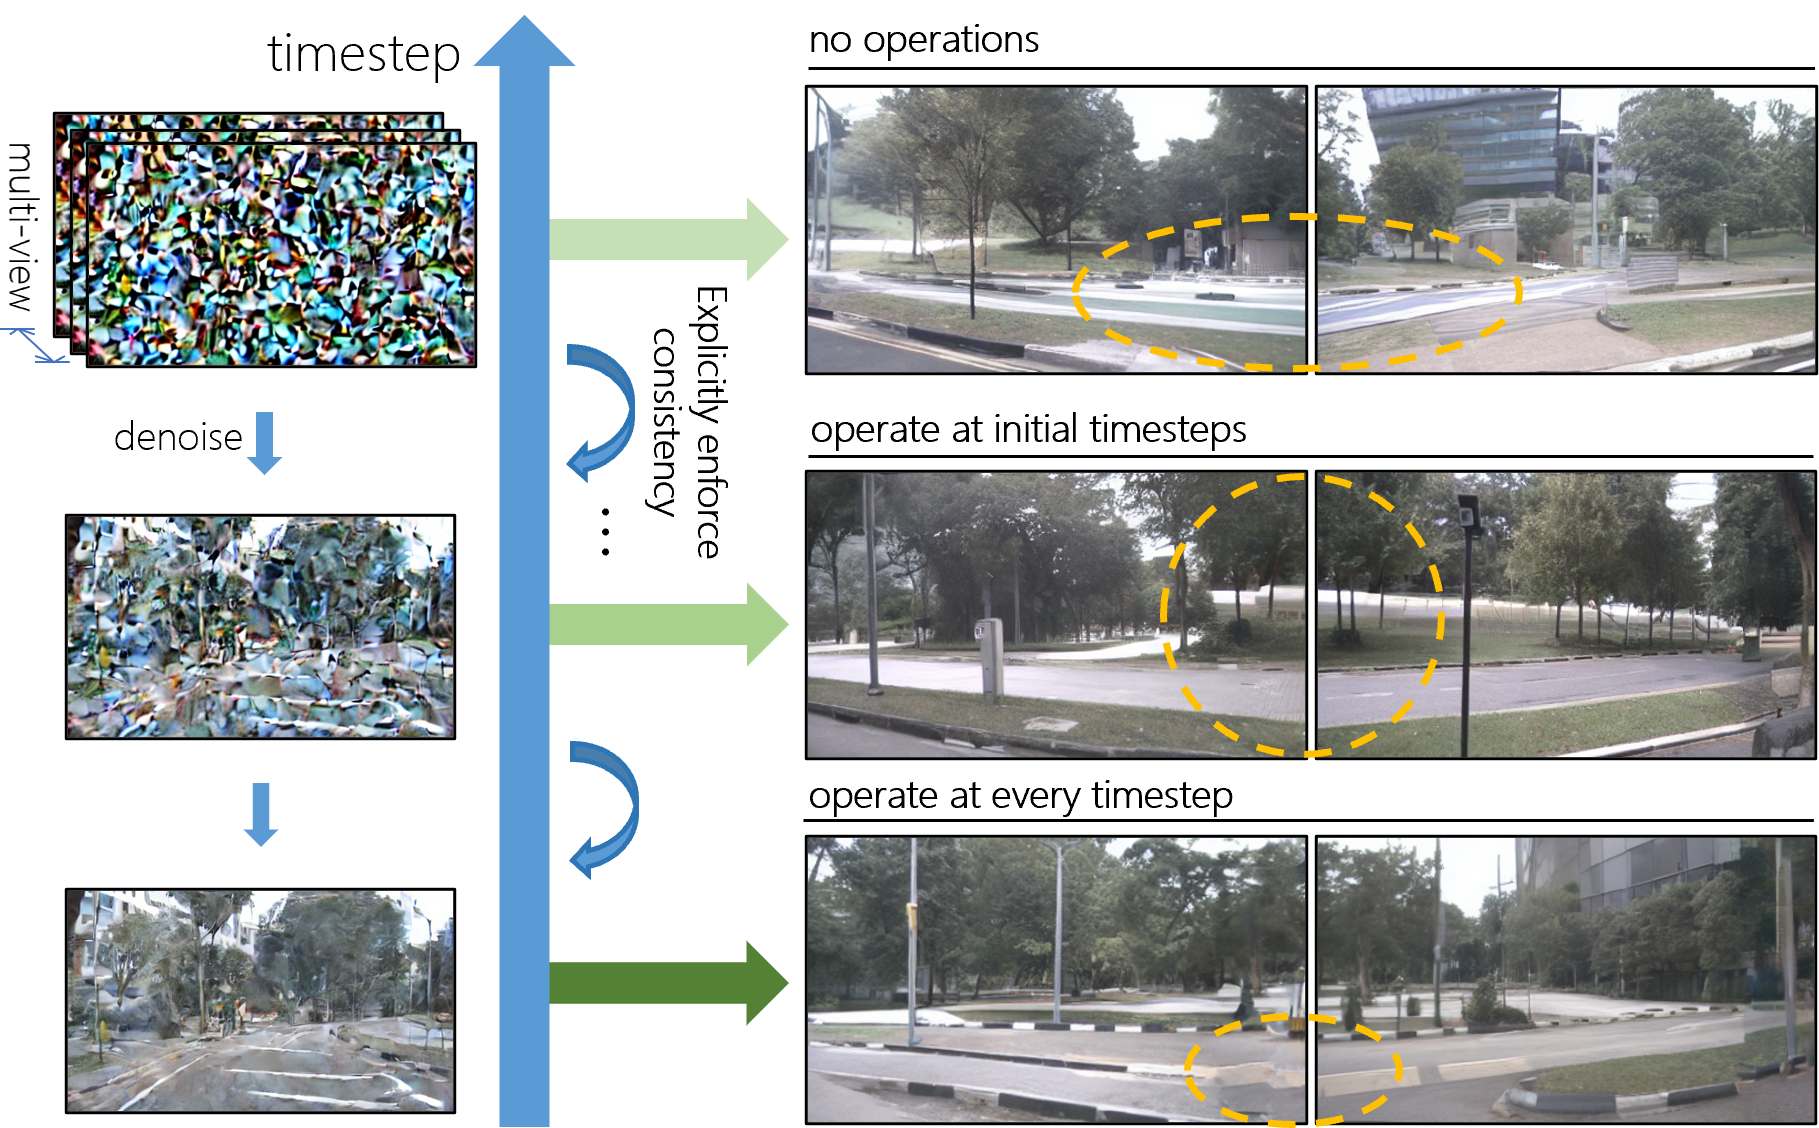
\includegraphics[width=\linewidth]{figures/explicit_enforce_consistency.png}
% \caption{By explicitly enforcing the consistency in latents during denoising process, we are able to obtain more visually consistent results at overlapping areas. 
% }
% \label{fig:denoise}
% \end{figure}

% \begin{figure}[ht]
% \centering
% \includegraphics[width=\linewidth]{figures/obj_control_method.jpg}
% \caption{Our method to achieve test-time controlability by combining multiple attention responses from paired instance masks and text description, in a training-free manner.
% }
% \label{fig:control_method}
% \end{figure}

\noindent{\textbf{Inference}} As claimed in above, MVPbev can be extended with instance-level controllability. Specifically, Our MVPbev allows the user to click on the target instance and provide color-specific requirements. To achieve this, we propose a special mechanism for multiple foreground objects control, which manipulates the response of cross-attention layers to accurately guide instance-level synthesis. Assuming that instance-level masks can be obtained at each view with either existing methods~\cite{cheng2022masked} or simple retrieval. Specifically, we first obtain the instance-level and scene-level latents individually with its paired prompt. Then they are effectively combined with those binary instance-level mask, leading to more spatial-consistent performance. 
%as paired text description and instance masks are passed to cross-attention layers, multiple instance-level prompts and one scene-level prompt that we already have are individually feed to certain cross-attention modules. Later on, instance masks are incorporated to effectively combine the response from those cross-attention modules, with text description and objects location aligned. In this way, it becomes possible to control multiple objects separately. 
Please note that such ability on foreground objects of MVPbev are training-free, leading to far better extendability and test-time controllability. We refer the readers to supplementary for more details.

% Specifically, as paired text description and instance masks are passed to cross-attention layers, multiple instance-level prompts and one scene-level prompt that we already have are individually feed to certain cross-attention modules. Later on, instance masks are incorporated to effectively combine the response from those cross-attention modules, with text description and objects location aligned. In this way, it becomes possible to control multiple objects separately. Please note that such ability on foreground objects of MVPbev are training-free, leading to far better extendability and test-time controllability 
% (See Fig.~\ref{fig:control_method})}

% \noindent{\textbf{Inference}} As claimed in above, MVPbev can be extended with instance-level controllability. Specifically, Our MVPbev allows the user to click on the target instance and provide color-specific requirements. To achieve this, we propose to denoise the background stuffs and foreground objects individually at initial denoising steps, then instance masks are incorporated as attentions to effective combine latents from both, finally the combined latents are denoised together. Please note that such ability on foreground objects of MVPbev are training-free, leading to far better extendability and test-time controllability (See Fig.~\ref{??})
\section{Experiment}
\label{sec:experiment}
% \subsection{Experiment setup}
\noindent{\textbf{Dataset}} We validate our ideas on NuScenes dataset~\cite{caesar2020nuscenes} where full 360-degree coverage provided by six cameras is available. Specifically, it consists of 1000 examples of street-view scenes in Boston and Singapore, each of which lasts for 20s and is captured at 12Hz. Besides 1.4M camera images, NuScenes also provides multi-modal data, including both global map layers and 3D object bounding boxes annotated on 40k keyframes. 
% NuScenes also provides multi-modal data, including LIDAR and RADAR sweeps, as well as map layers. More importantly, 3D object bounding boxes are annotated 40k keyframes. 
We follow the standard split of 700/150/150 for training, validation, and testing. We report our results on the validation set of Nuscenes and follow the split of~\cite{caesar2020nuscenes} where 600 sets of images are used. 

\begin{table*}[h!]
    \centering
    \caption{Quantitative results and human analysis on NuScenes. We observe a noticeable superiority of our MVPbev. %over existing methods.
    % Numbers show the winning percent of left column methods vs top row methods 
    }
    \resizebox{\textwidth}{!}{
    
% \subfloat[Quantitative results on NuScenes dataset]{
% \begin{tabular}{c|ccc|c|c} 
% \hline
% \multirow{2}{*}{Method} & \multicolumn{3}{c|}{Image Quality} & Semantics Consistency & Visual Consistency \\ 
% \cline{2-6}
%  & FID$\downarrow$ & IS$\uparrow$ & CS$\uparrow$ & $\rm{IoU_{BEV}}$$\uparrow$ & PSNR$\uparrow$ \\ 
% \hline
% Reference-score & $18.87$ & $ 4.53 $ & $25.94$ & $0.711$ & $15.37$ \\ 
% Controlnet~\cite{zhang2023adding} & $21.93$ & $4.71$ & $27.02$ & $0.434$ & $12.82$ \\ 
% MVD~\cite{Tang2023mvdiffusion} & $19.89$ & $4.91$ & $27.07$ & $0.440$ & $12.66$ \\
% BEVGen\cite{swerdlow2023street} & $25.54$ & - & - & $0.502$ & - \\
% MagicDrive\cite{gao2023magicdrive} & $\mathbf{16.20} $ & - & - & $\mathbf{0.611}$ & - \\
% \hline
% Ours & $16.95$ & $\mathbf{6.35}$ & $\mathbf{28.79}$ & 0.510 & $\mathbf{20.67}$ \\
% \hline
% \end{tabular}
% }

\subfloat[Quantitative results on NuScenes dataset]{
\begin{tabular}{c|c|ccc|c|c} 
\hline
\multirow{2}{*}{Method} & \multirow{2}{*}{Training Samples} & \multicolumn{3}{c|}{Image Quality} & Semantics Consistency & Visual Consistency \\ 
\cline{3-7}
 & & FID$\downarrow$ & IS$\uparrow$ & CS$\uparrow$ & $\rm{IoU_{BEV}}$$\uparrow$ & PSNR$\uparrow$ \\ 
\hline
Reference-score & - &$6.20$ & $ 5.77 $ & $27.54$ & $0.711$ & $15.37$ \\ \hline \hline
BEVGen\cite{swerdlow2023street} & $28130$ & $25.54$ & - & - & $0.502$ & - \\
MagicDrive\cite{gao2023magicdrive} & $28130$ & $\mathbf{16.20} $ & - & - & $\mathbf{0.611}$ & - \\ \hline
Controlnet~\cite{zhang2023adding} & $6000$ & $21.93$ & $4.71$ & $27.02$ & $0.434$ & $12.82$ \\ 
MVD~\cite{Tang2023mvdiffusion} & $6000$ & $19.89$ & $4.91$ & $27.07$ & $0.440$ & $12.66$ \\
\hline \hline
Ours & $6000$ & $16.95$ & $\mathbf{6.35}$ & $\mathbf{28.79}$ & 0.510 & $\mathbf{20.67}$ \\
\hline
\end{tabular}
}


\quad

\subfloat[Human analysis on NuScenes dataset. ]{
\begin{tabular}{cc|ccc}
\hline
\multicolumn{2}{c|}{Comparisons}                                                                                              & Win & Undecided & Lose \\ \hline \hline
\multicolumn{1}{c|}{\multirow{3}{*}{\begin{tabular}[c]{@{}c@{}}Cross-view\\ Consistency\end{tabular}}} & MVD v.s. Controlnet  & $\mathbf{.26}$ & $.50$       & $.25$  \\
\multicolumn{1}{c|}{}                                                                                  & Ours v.s. Controlnet & $\mathbf{.73}$ & $.27$       & $.00$  \\
\multicolumn{1}{c|}{}                                                                                  & Ours v.s. MVD        & $\mathbf{.71}$ & $.29$       & $.00$  \\ \hline \hline
\multicolumn{1}{c|}{\begin{tabular}[c]{@{}c@{}}Camera Pose\\ Consistency\end{tabular}}                 & Ours v.s. MagicDrive & $\mathbf{.61}$ & $.31$       & $.08$    \\ \hline
\end{tabular}
}

% \subfloat[Human analysis on NuScenes dataset. ]{
% \begin{tabular}{c|c|ccc}
%     \toprule
%     \multicolumn{2}{c|}{Comparisons} & Win & Undecided & Loss \\
%     \midrule
%     \multirow{3}{}{Cross-view consistency}
%     MVD~\cite{Tang2023mvdiffusion} v.s. Controlnet~\cite{zhang2023adding} & .26 & .50 & .25 \\
%     Ours v.s. Controlnet~\cite{zhang2023adding} & .73 & .27 & .00 \\
%     Ours v.s. MVD~\cite{Tang2023mvdiffusion} & .71 & .29 & .00 \\
%     \hline 
    
% \end{tabular}
% }


% original table 1
% \begin{table*}%[H]
%            \centering
%            \captionsetup[subtable]{position = below}
%           \captionsetup[table]{position=top}
%            \caption{Blahblah}
%            \begin{subtable}{0.3\linewidth}
%                \centering
%                \begin{tabular}{|c|c|}
%                    \hline
%                    \textbf{h [m]} & \textbf{dim [m]} \\ \hline
%                    30 & 0.75 \\ \hline
%                    50 & 1.25 \\ \hline
%                    70 & 1.75 \\ \hline
%                    100 & 2.50 \\ \hline
%                \end{tabular}
%                \caption{Minimum dimension of an object for it to be detected by the FFT algorithm at different heights}
%                \label{tab:dimFFT}
%            \end{subtable}%
%            \hspace*{4em}
%            \begin{subtable}{0.3\linewidth}
%                \centering
%                \begin{tabular}{|c|c|}
%                    \hline
%                    \textbf{h [m]} & \textbf{dim [m]} \\ \hline
%                    30 & 0.28 \\ \hline
%                    50 & 0.47 \\ \hline
%                    70 & 0.66 \\ \hline
%                    100 & 0.94 \\ \hline
%                \end{tabular}
%                 \caption{Minimum dimension of an object for it to be detected by the GMM algorithm at different heights}
%                  \label{tab:dimGMM}
%            \end{subtable}
%        \end{table*}


% %% side by side using parbox
% \parbox{.45\linewidth}{
% \centering

% \begin{tabular}{c|ccc|cc|c} 
% \hline
% \multirow{2}{*}{Method} & \multicolumn{3}{c|}{Image Quality} & \multicolumn{2}{c|}{Semantics Consistency} & Visual Consistency \\ 
% \cline{2-7}
%  & FID$\downarrow$ & IS$\uparrow$ & CS$\uparrow$ & $\rm{IoU_{Pers}}$$\uparrow$ & $\rm{IoU_{BEV}}$$\uparrow$ & PSNR$\uparrow$ \\ 
% \hline
% Reference-score & $18.87$ & $ 5.11 $ & $26.46$ & $0.618$ & $0.711$ & $15.37^*$ \\ 
% SD + Controlnet~\cite{??} & $\mathbf{32.71}$ & $\mathbf{3.53}$ & $28.66$ & $0.476$ & $0.366$ & $12.08$ \\ 
% MVDiffusion~\cite{??} & $43.83$ & $3.11$ & $28.69$ & $0.560$ & $0.418$ & $11.64$ \\ 
% \hline
% Ours & $38.22$ & $3.25$ & $\mathbf{28.71}$ & $\mathbf{0.588}$ & $\mathbf{0.421}$ & $\mathbf{20.05}$ \\
% \hline
% \end{tabular}

% \caption{1. xxxxxxxxxxxxxxxxxxxxxx}
% }

% \hfill


% \parbox{.45\linewidth}{
% \centering

% \begin{tabular}{c|ccc}
%     \toprule
%      Comparisons & Win & Undecided & Loss \\
%     \midrule
%     MVDiffusion~\cite{??} v.s. SD + Controlnet~\cite{??} & .26 & .50 & .25 \\
%     Ours v.s. SD + Controlnet~\cite{??} & .73 & .27 & .00 \\
%     Ours v.s. MVDiffusion~\cite{??} & .71 & .29 & .00 \\
%     \hline 
    
% \end{tabular}

% \caption{2. xxxxxxxxxxxxxxxxxxx}
% }
    }
    \label{tbl:qualitative}
\end{table*}

\begin{figure*}[t]
\centering
\includegraphics[width=0.95\linewidth]{figures/qualitative_comparison.png}
\caption{Our MVPbev is able to achieve the most visual and semantic consistent images w.r.t. input control signal. We highlight the overlapping area and road boundary in orange bounding boxes and green lines. 
}
\label{fig:quali_comp}
\end{figure*}

\noindent{\textbf{Evaluation metrics}} We follow~\cite{Tang2023mvdiffusion} to include the image quality of generated images and their visual consistency in our evaluation metrics. In addition, semantic consistency is also valued to reflect the synthesis quality of different semantic categories.

\begin{packed_lefty_item}
\item \textit{Image quality} is measured by Fréchet Inception Distance (FID)~\cite{cortes2015advances}, Inception Score (IS)~\cite{salimans2016improved}, and CLIP Score (CS)~\cite{radford2021learning}. In particular, FID is based on the distribution similarity between the features of the generated and real images. The IS measures the diversity and predictability of generated images. Finally, CS measures the text-image similarity according to pre-trained CLIP models~\cite{radford2021learning}.

\item \textit{Visual consistency} provides pixel-wise similarity measurements on overlapping regions. We borrow the idea from Peak Signal-to-Noise Ratio (PSNR) where we first compute this PSNR between all the overlapping regions, and then compare this “overlapping PSNR” for ground truth images and generated images. The higher this value is, the better visual consistency will be. Note that the process of computing "overlapping PSNR" is based on estimated homography matrices, it's possible that generated image yields higher values than the ground truth image.

\item \textit{Semantic consistency} measures the pixel-wise semantic consistency between generated images and ground truth. In our case, we utilize the Intersection-over-Union (IoU) score. Particularly, we report the semantic IoU both in perspective view and BEV. As for the former, we apply pre-trained segmentation model~\cite{cheng2022masked} on generated images, leading to semantic predictions in perspective view. These predictions are then compared with $\{S_m\}_m$ to obtain IoU in perspective view. As for the latter, we apply pre-trained CVT~\cite{zhou2022cross} to generated images and the BEV IoU is obtained by comparing predictions from CVT with $\textit{B}$.

\item \textit{Object-level controllability} measures how accurately the object-instance is generated w.r.t. test-time descriptions. Here we report the averaged color distance Delta-E in CIELAB color space as well as their standard deviations.  
\end{packed_lefty_item}

Besides these metrics, we also perform human analysis. We request humans to decide which method is more visually realistic and consistent when results from different methods are provided. %Please note that 
Methods are anonymous to humans and when compared. And we ensure that the same input control signals are provided to various methods. Meanwhile, we also conduct experiments with instance-level controllability. Humans are provided with objects as well as their targeted color, paired with the generated images. And they will vote on whether the generated objects meet the requirements.
% Specifically, given the same input control signal, we can obtain multi-view images from all methods. Humans are fed with two sets of generated images from two different methods and then asked to make pairwise comparisons about which set is better, based on their visual qualities. 

\begin{figure*}[t]
\centering
\includegraphics[width=0.95\linewidth]{figures/demo.png}
\caption{Qualitative results of MVPbev. We provide three sets of examples. The leftmost column consists of input signals, while the 2nd to 7th columns are images from different perspective views.
}
\label{fig:demo}
\end{figure*}

\noindent{\textbf{Baselines}} We select the following four state-of-the-art methods as our baselines for thorough comparisons:
\begin{packed_lefty_item}
\item \textit{SD+ControlNet}~\cite{rombach2021highresolution, zhang2023adding} is a basic yet powerful image generation model. Specifically, we work on the projected $\{S_m\}_m$ to avoid domain gaps from different viewpoints. Starting from a pre-trained ControlNet~\cite{zhang2023adding}, this baseline is fine-tuned on NuScenes training.  
\item \textit{MVDiffusion}~\cite{Tang2023mvdiffusion} is proposed to generate multi-view consistent images. % and achieves good performance on tasks like panoramic image generation. 
However, it is designed neither for dramatic view changes, e.g., BEV to perspective view, nor for semantic control signals. To this end, we %follow our pipeline to 
first map BEV semantics to perspective view and then update MVDiffusion with a pre-trained ControlNet~\cite{zhang2023adding} backbone. Specifically, We re-implement~\cite{Tang2023mvdiffusion} based on its official code and fine-tune it on NuScenes training images.
\item \textit{BEVGen}~\cite{swerdlow2023street} is the first step towards road scene generation, where the control signals are limited to BEV semantics and camera parameters. The full dataset is used for training. % And $28130$ set of images are used for training purposes.   
\item \textit{MagicDrive}~\cite{gao2023magicdrive}is the most recent published work on road scene generation. We use their released model for efficient comparison. Please note that we use only $20\%$ images uniformly sampled from dataset for training while they use the full dataset. % in their official implementation.
\end{packed_lefty_item}
% These four methods are chosen for performance and re-productivity purposes. We refer the readers to supplementary for full implementation details.

\subsection{Implementation Details}
Our BEV semantics $\textit{B}$ reflects an 80m $\times$ 80m space with ego car located at the center position. $c_b$ represents the drivable area in NuScenes. The resolution of the perspective image is $H\times W = 256\times 448$, leading to $h\times w = 32\times56$. As for the hyper-parameters, we set $M$ and $K$ to 6 and 3 respectively. We have implemented the system with PyTorch~\cite{paszke2019pytorch} while using publicly available Stable Diffusion codes~\cite{von-platen-etal-2022-diffusers}. Specifically, it consists of a denoising UNet to execute the denoising process within a compressed latent space and a VAE to connect the image and latent spaces. The pre-trained VAE of the Stable Diffusion is maintained with official weights and is used to encode images during the training phase and decode the latent codes into images during the inference phase. In experiments, we use a machine with 1 NVIDIA A40 GPU for training and inference. Batch size is set to 6 and $T$ equals to 50. We refer the readers to supplementary for full implementation details.

% \begin{figure*}[h]
% \centering
% \includegraphics[width=\linewidth]{figures/fixed_bev_prompt_control.png}
% \caption{We are able to generate photo-realistic, diverse yet consistent multi-view perspective images with various control signals.
% }
% \label{fig:controllability}
% \end{figure*}

\begin{figure*}[t]
\centering
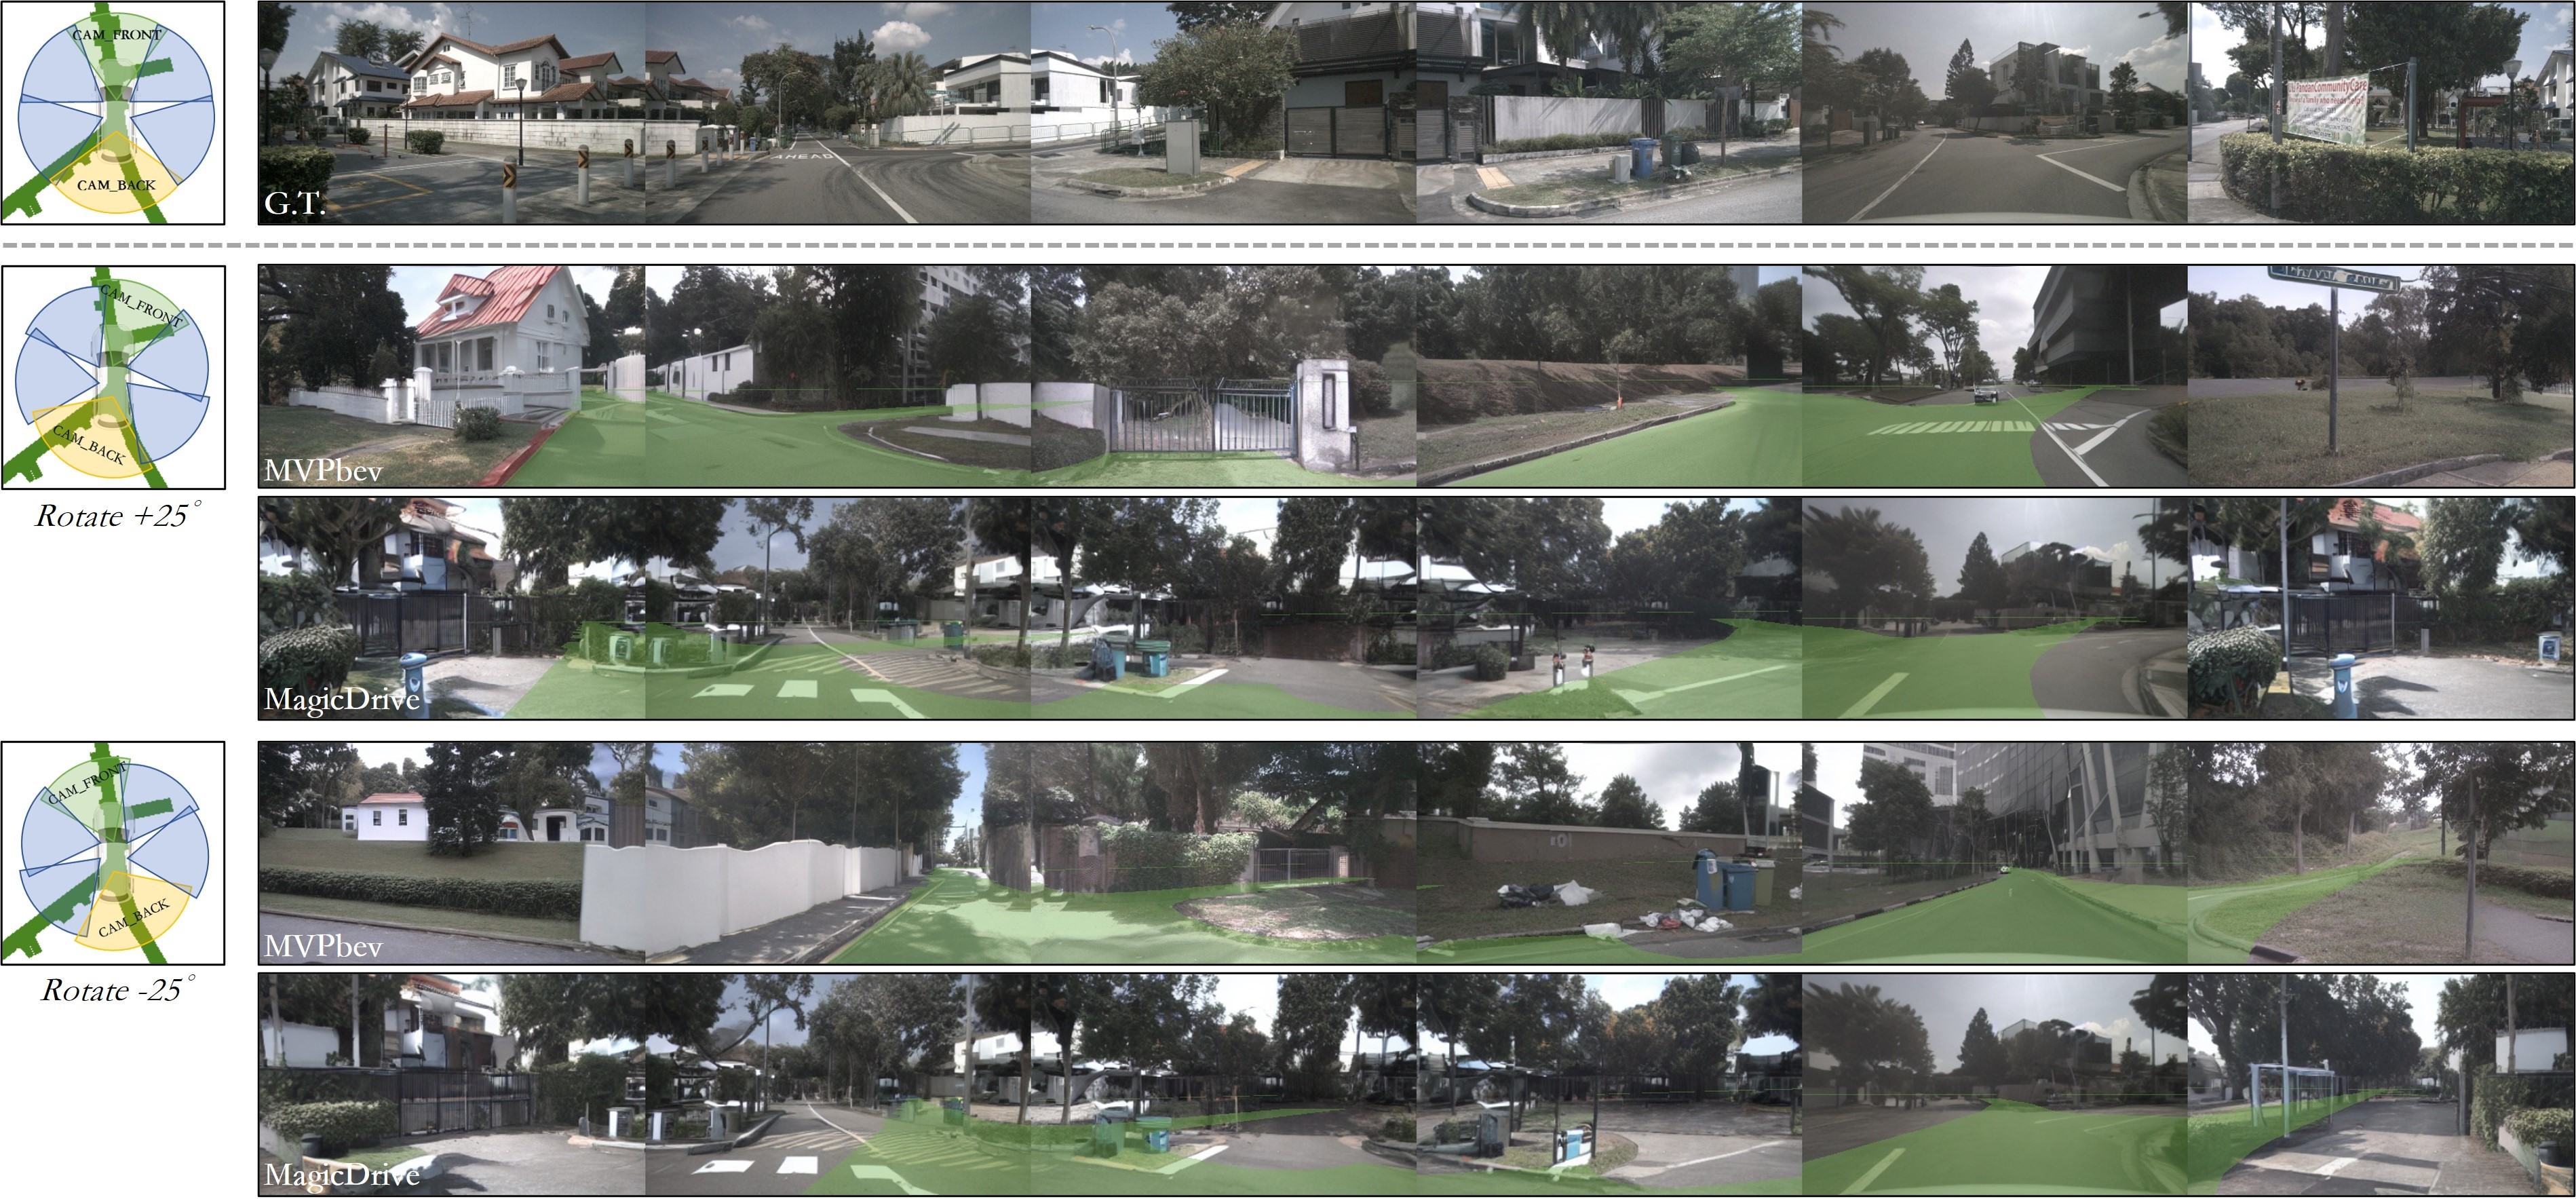
\includegraphics[width=0.95\linewidth]{figures/camera_pose_demo_semantic_overlay.jpg}
\caption{MVPbev is robust to camera pose changes without re-train the entire model, providing better test-time generalizability.
}
\label{fig:view_point}
\end{figure*}

\begin{figure}[h]
\centering
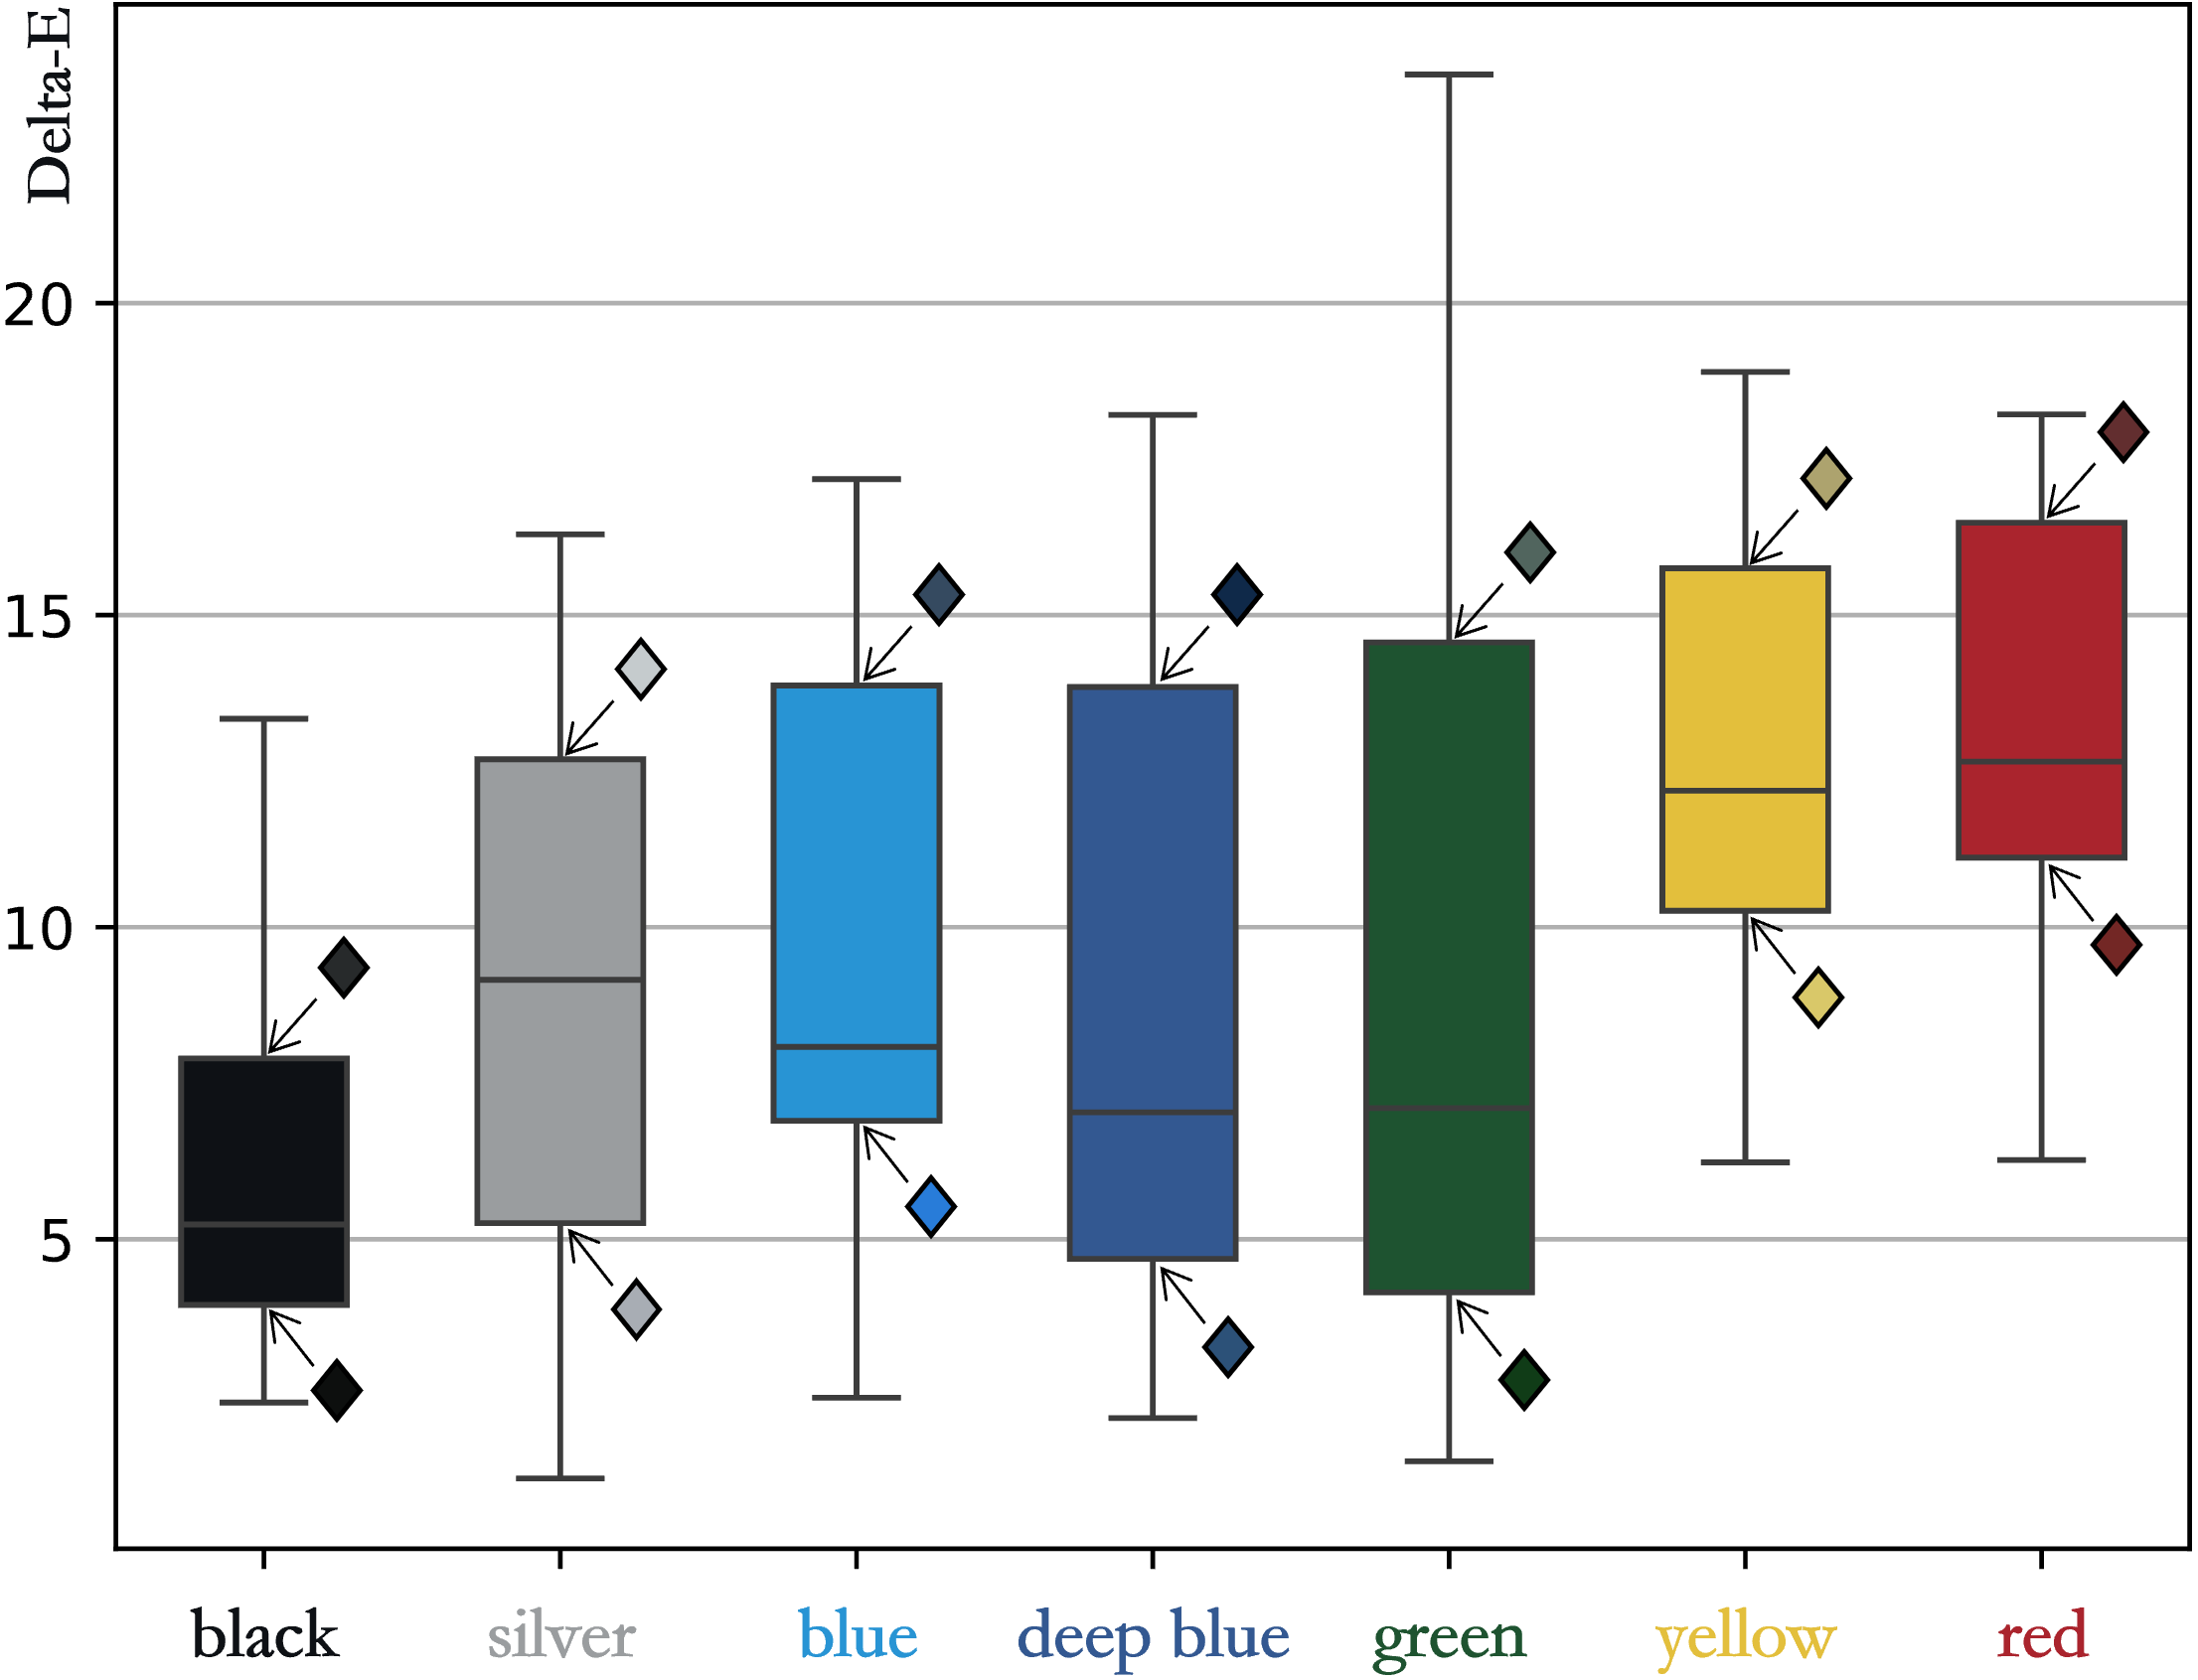
\includegraphics[width=0.9\linewidth]{figures/color_boxfig.png}
\caption{The Delta-E distance between the ground truth and generated color on our controlled instances.
}
\label{fig:obj_instance_eval}
\vspace{-2mm}
\end{figure}

\begin{figure}[b]
\centering
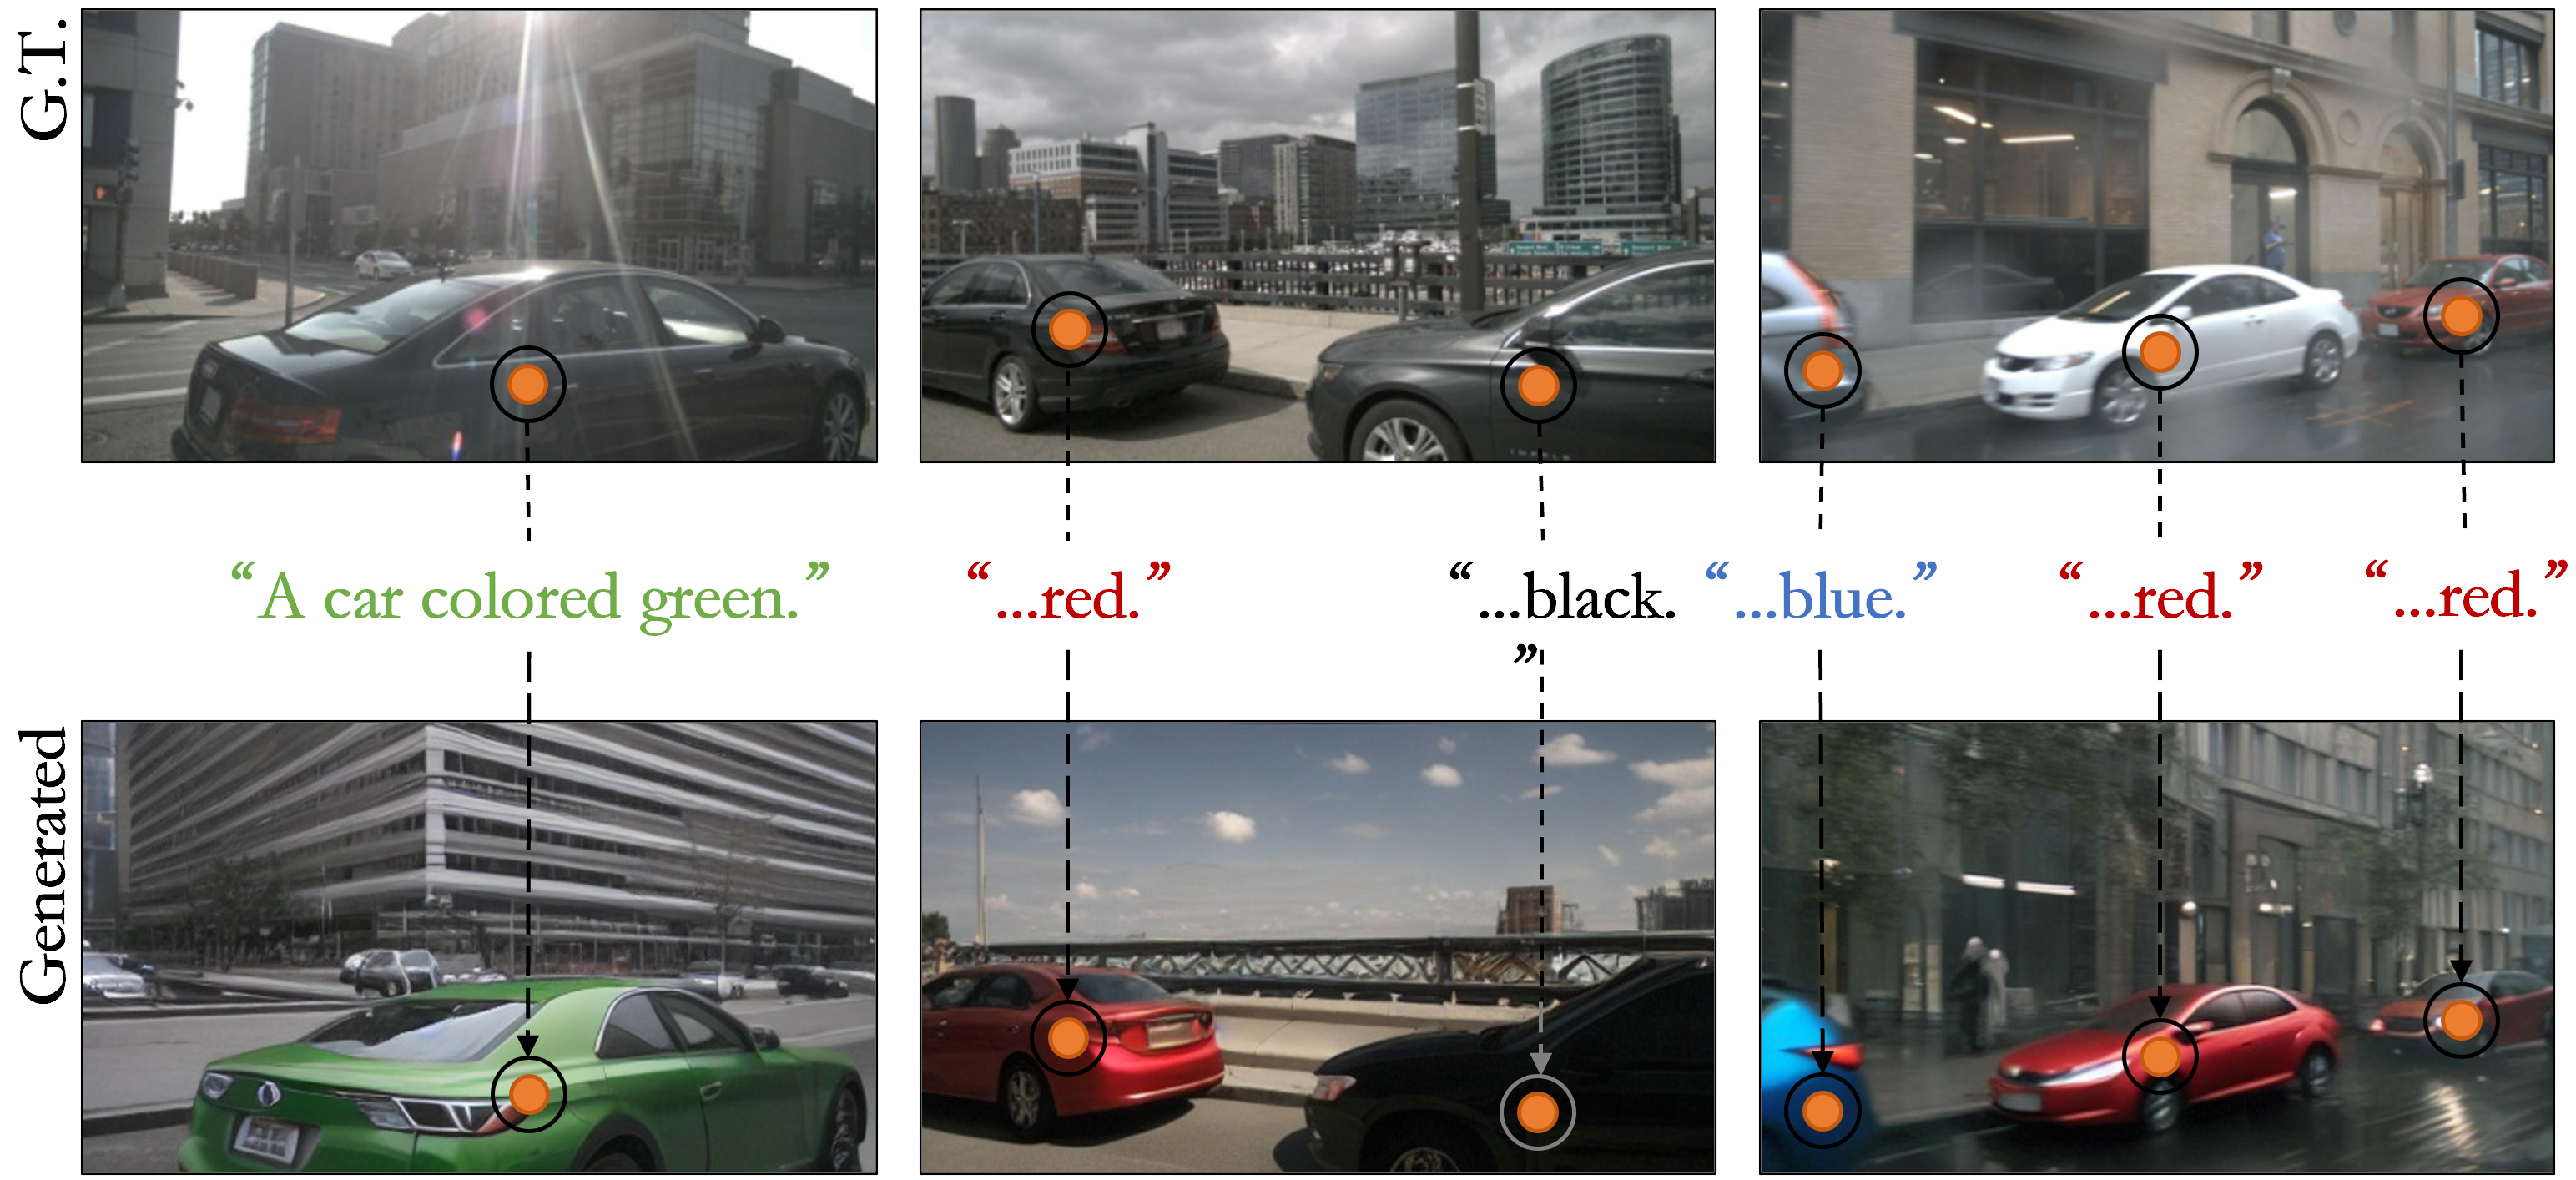
\includegraphics[width=0.9 \linewidth]{figures/mulit_obj_color_control_demo.png}
\caption{MVPbev is able to handle test-time instance-level controllability with various color requests.
}
\label{fig:obj_instance}
\end{figure}
\subsection{Multi-view BEV generation}
We compare our MVPbev with baselines and report the performance in Table~\ref{tbl:qualitative}. The first row in this table is obtained on ground truth images. For instance, we split the ground truth validation images into two halves, and then obtain the FID score by taking one split as ground truths and the other half as generated images. As for the IoU scores, we apply the Mask2Former~\cite{cheng2022masked} and CVT~\cite{zhou2022cross} on validation images and compare their predictions with ground truths $\{S_m\}_m$ and $\textbf{B}$. As can be found in this table, our MVPbev almost always ranks first among comparable baselines, such as Controlnet and MVD. And we even achieve comparable results w.r.t. SOTA methods that are trained with far more training data.
% More importantly, it even outperforms the ground truth by a large margin with PSNR. Such observation further validates our claim that consistency can be effectively enforced in overlapping areas.

We also provide visual comparisons to existing baselines in Fig.~\ref{fig:quali_comp}. The top row showcases the bev semantics $\textit{B}$ as well as the projected semantics $\{S_m\}_{m=1}^M$ in perspective views. We also provide the ground truths as well as multi-view images generated by other methods from the second to the fifth row. Our method MVPbev, compared to other baselines, produces the most consistent perspective images, especially at overlapping FOVs. As highlighted by orange bounding boxes and green lines, our MVPbev not only generates perspective images that are consistent with semantic guidance, but also maintains high visual consistency across multiple views. Such consistency is more visible and valuable for pixels that appear in different views.

\noindent{\textbf{Qualitative results}}
Besides quantitative results, we also provide qualitative examples in Fig.~\ref{fig:demo}. As can be found in this figure, our MVPbev is able to generate visually consistent images from diverse bev semantics and text prompts. Compared to ground truth, ours can obtain satisfactory consistency at overlapping FOVs. We refer the readers to supplementary for more visual examples about the controllability over BEV and text prompt.
% , which is consistent with the PSNR score.

% \noindent{\textbf{Controllability over BEV and text prompts}} is one of the main goals of our paper. Ideally, a good generative model should be capable of handling various BEVs with diverse text prompts. To this end, we showcase the controllability of MVPbev from the above-mentioned two perspectives and provide visual examples in Fig.~\ref{fig:controllability}. As can be found in this figure, we are able to generate photo-realistic, diverse yet consistent multi-view perspective images with different control signals.
% \vspace{-4mm}
\noindent{\textbf{Test-time controllability and generalizability}} \textit{View-point generalizability} As described before, one of the main drawbacks of the existing work is the lack of ability in terms of handling view-point changes at test time. 
%In contrast, our MVPbev is free of such problems as it decouples the view projection and scene generation. 
To showcase our ability, we revise the camera extrinsic during inference and check whether the results would change accordingly. In practice, we rotate the all $M$ camera by $\{-25^{\circ},-15^{\circ},-5^{\circ},5^{\circ},15^{\circ},25^{\circ}\}$ w.r.t. the head direction of the ego car, mimicking potential different setups of camera mounting. This is equivalent to changing the $\{R_m\}_m$ in our input signal. We randomly generate 200 sets of images for each rotation angle and provided the generated results from MagicDrive~\cite{gao2023magicdrive} and ours to humans. Qualitative results are provided in Fig.~\ref{fig:view_point}. We overlay the projected semantics in each view for better visualization. Not surprisingly, prior art merely follows the control signal. While MVPbev gives superior results considering the semantics, demonstrating better test-time generalizability. And this observation is also supported by our detailed human analysis in Table~\ref{tbl:qualitative}.

\noindent{\textit{Object-level controllability}} A practical generative model should be a controllable one. To this end, we conduct another experiment to showcase the object-level controllability. In this experiment, we include an additional description of the object color in the original text prompt and then check whether such control can be reflected in generated scenes at test time. In experiment, we randomly choose 151 set of images, including 195 object instances, and provide random color requests out of seven popular colors for vehicles.
We report our qualitative evaluations in Fig.~\ref{fig:obj_instance_eval} and qualitative examples in Fig.~\ref{fig:obj_instance} respectively. Though the Delta-E seems to be noticeable, we argue that this is mainly due to the de-noising process where colors of vehicles are in harmony with the environment, e.g., less bright in rainy days. This is supported by our visual results as well as human analysis. 
% In general, we are able to achieve good instance-level controllability, which is beyond prior art. 

% As demonstrated before, our MVPbev is capable of generating multi-view consistent perspective images from BEV semantics. One might notice from our visual examples that it mainly focuses on background layouts, ignoring foreground road participants. In practice, we can further extend our MVPbev by incorporating vehicles. Specifically, we include the 3D object information as well as their visibility into account. At the projection stage, objects are mapped to 2D perspective view if they are visible. We then fine-tune our multi-view LDM such that an additional $c_b$ can be introduced as control signals. We refer the readers to supplementary for more details as well as qualitative results on objects.
\noindent{\textbf{Human analysis}}
Compared to evaluation metrics, human analysis provides a more reliable tool for image quality measurement. Therefore, we conduct a comprehensive human analysis of our tasks. Specifically, we provide two sets of generated images, which are generated from two different methods with the same input signal, to humans. Then we ask them to decide which set of images is better, considering the image quality and visual consistency. %We also allow humans to label them as 'undecided' but this option is not encouraged. 
As can be found in Table~\ref{tbl:qualitative}, our MVPbev outperforms baselines significantly, indicating that we can indeed generate photo-realistic yet consistent images. Meanwhile, we report the test-time view-point changes by comparing ours to MagicDrive~\cite{gao2023magicdrive}, showing that MVPbev provides better generalizability quantitatively. Finally, we ask humans to decide whether the generated instance color can be regarded as the requested one. In our experiment, 93.5$\%$ of the instances are voted as correctly generated. We refer the readers to supplementary for more details about human analysis.

% In particular, we have conducted two sets of experiments, including comparisons between baselines and MagicDrive~\cite{gao2023magicdrive}. As can be found in Tab.~\ref{tbl:qualitative}, our MVPbev outperforms baselines significantly, indicating that we can indeed generate photo-realistic yet consistent images. Meanwhile, we report the test-time view-point changes by comparing ours to MagicDrive~\cite{gao2023magicdrive}. In practice, our MVPbev allows more generalizability quantitatively compared to prior art. We refer the readers to supplementary for more details about human analysis.

% As can be found in Tab.~\ref{tbl:qualitative}, our MVPbev outperforms baselines significantly, indicating that we can indeed generate photo-realistic yet consistent images.~\textcolor{red}{We further ask the humans to compare}

% \begin{table}[t!]
%     \centering
%     % \resizebox{5cm}{
%     \begin{tabular}{c|ccc}
    \toprule
     Comparisons & Win & Undecided & Lose \\
    \midrule
    MVD v.s. base & .26 & .50 & .25 \\
    Ours v.s. base & .73 & .27 & .00 \\
    \hline 
    Ours v.s. MVD & .71 & .29 & .00 \\
    \hline 
    
\end{tabular}
%     % }
%     \caption{Human analysis on NuScenes validation images.
    
%     %on Pascal under R2-5. We colored results under white and black settings in red and blue respectively. For instance, the bottom-left 0.78 means that $78\%$ of GLOW results are voted to be better than TOG~\cite{chow2020adversarial} by humans. 
    
%     % Numbers show the winning percent of left column methods vs top row methods 
%     }
%     \label{tbl:human}
% \end{table}

% We give an example image in Fig.~\textcolor{red}{\ref{??}} and refer to the readers to supplementary for more details.

%\vspace{-4mm}
\section{Conclusion}
\label{sec:conclusion}
%\vspace{-2mm}
Our goal is to generate multi-view perspective RGB from text prompts given BEV semantics. To this end, we introduce a two-stage method MVPbev to first project BEV semantics to perspective views and then perform image generation w.r.t. both text prompts and individual perspective semantics. Specifically, we propose a novel initialization and denoising processes to explicitly enforce local consistency at overlapping FOVs. Results showcase the superiority of MVPbev under various metrics and test-time generalizability.

% multi-view attention module to implicitly leverage global consistency w.r.t. camera homography among views, followed by
\begin{acks}
This work was supported in part by the National Natural
Science Foundation of China (No. 62125201, 62020106007)
\end{acks}


\bibliographystyle{ACM-Reference-Format}
\balance
\bibliography{main}

% \appendix
% %%
%% This is file `sample-authordraft.tex',
%% generated with the docstrip utility.
%%
%% The original source files were:
%%
%% samples.dtx  (with options: `authordraft')
%% 
%% IMPORTANT NOTICE:
%% 
%% For the copyright see the source file.
%% 
%% Any modified versions of this file must be renamed
%% with new filenames distinct from sample-authordraft.tex.
%% 
%% For distribution of the original source see the terms
%% for copying and modification in the file samples.dtx.
%% 
%% This generated file may be distributed as long as the
%% original source files, as listed above, are part of the
%% same distribution. (The sources need not necessarily be
%% in the same archive or directory.)
%%
%% Commands for TeXCount
%TC:macro \cite [option:text,text]
%TC:macro \citep [option:text,text]
%TC:macro \citet [option:text,text]
%TC:envir table 0 1
%TC:envir table* 0 1
%TC:envir tabular [ignore] word
%TC:envir displaymath 0 word
%TC:envir math 0 word
%TC:envir comment 0 0
%%
%%
%% The first command in your LaTeX source must be the \documentclass command.
% \documentclass[sigconf,authordraft]{acmart}
\documentclass[sigconf]{acmart}
%% NOTE that a single column version may required for 
%% submission and peer review. This can be done by changing
%% the \doucmentclass[...]{acmart} in this template to 
%% \documentclass[manuscript,screen]{acmart}
%% 
%% To ensure 100% compatibility, please check the white list of
%% approved LaTeX packages to be used with the Master Article Template at
%% https://www.acm.org/publications/taps/whitelist-of-latex-packages 
%% before creating your document. The white list page provides 
%% information on how to submit additional LaTeX packages for 
%% review and adoption.
%% Fonts used in the template cannot be substituted; margin 
%% adjustments are not allowed.
\usepackage{amsmath}
%%
%% \BibTeX command to typeset BibTeX logo in the docs
\AtBeginDocument{%
  \providecommand\BibTeX{{%
    \normalfont B\kern-0.5em{\scshape i\kern-0.25em b}\kern-0.8em\TeX}}}

\settopmatter{printacmref=false} % Removes citation information below abstract
\renewcommand\footnotetextcopyrightpermission[1]{} % removes footnote with conference information in first column
\pagestyle{plain} % removes running headers 
\setcopyright{none}

%% These commands are for a PROCEEDINGS abstract or paper.
% \acmConference[Conference acronym 'XX]{Make sure to enter the correct
%   conference title from your rights confirmation emai}{June 03--05,
%   2018}{Woodstock, NY}
%
%  Uncomment \acmBooktitle if th title of the proceedings is different
%  from ``Proceedings of ...''!
%
%\acmBooktitle{Woodstock '18: ACM Symposium on Neural Gaze Detection,
%  June 03--05, 2018, Woodstock, NY} 
% \acmISBN{978-1-4503-XXXX-X/18/06}


%%
%% Submission ID.
%% Use this when submitting an article to a sponsored event. You'll
%% receive a unique submission ID from the organizers
%% of the event, and this ID should be used as the parameter to this command.
% \acmSubmissionID{xxxx}

%%
%% For managing citations, it is recommended to use bibliography
%% files in BibTeX format.
%%
%% You can then either use BibTeX with the ACM-Reference-Format style,
%% or BibLaTeX with the acmnumeric or acmauthoryear sytles, that include
%% support for advanced citation of software artefact from the
%% biblatex-software package, also separately available on CTAN.
%%
%% Look at the sample-*-biblatex.tex files for templates showcasing
%% the biblatex styles.
%%

%%
%% For managing citations, it is recommended to use bibliography
%% files in BibTeX format.
%%
%% You can then either use BibTeX with the ACM-Reference-Format style,
%% or BibLaTeX with the acmnumeric or acmauthoryear sytles, that include
%% support for advanced citation of software artefact from the
%% biblatex-software package, also separately available on CTAN.
%%
%% Look at the sample-*-biblatex.tex files for templates showcasing
%% the biblatex styles.
%%

%%
%% The majority of ACM publications use numbered citations and
%% references.  The command \citestyle{authoryear} switches to the
%% "author year" style.
%%
%% If you are preparing content for an event
%% sponsored by ACM SIGGRAPH, you must use the "author year" style of
%% citations and references.
%% Uncommenting
%% the next command will enable that style.
%%\citestyle{acmauthoryear}

%%
%% end of the preamble, start of the body of the document source.
\begin{document}

%%
%% The "title" command has an optional parameter,
%% allowing the author to define a "short title" to be used in page headers.
\title{Supplementary Materials: \\ MVPbev: Multi-view Perspective Image Generation from BEV with Test-time Controllability and Generalizability}

%%
%% The "author" command and its associated commands are used to define
%% the authors and their affiliations.
%% Of note is the shared affiliation of the first two authors, and the
%% "authornote" and "authornotemark" commands
%% used to denote shared contribution to the research.
% \author{Ben Trovato}
% \authornote{Both authors contributed equally to this research.}
% \email{trovato@corporation.com}
% \orcid{1234-5678-9012}
% \author{G.K.M. Tobin}
% \authornotemark[1]
% \email{webmaster@marysville-ohio.com}
% \affiliation{%
%   \institution{Institute for Clarity in Documentation}
%   \streetaddress{P.O. Box 1212}
%   \city{Dublin}
%   \state{Ohio}
%   \country{USA}
%   \postcode{43017-6221}
% }

% \author{Anonymous Authors}
\author{Buyu Liu}\authornote{Equal contribution}\affiliation{\institution{Harbin Institute of Technology (Shenzhen)}
  \country{China}}
  \email{buyu.liu@zju.edu.cn}
\author{Kai Wang}\authornotemark[1]\affiliation{\institution{Hangzhou Dianzi University}\country{China}}
\email{21052222@hdu.edu.cn}
\author{Yansong Liu}
\affiliation{\institution{Hangzhou Dianzi University}\country{China}}
\email{19011121@hdu.edu.cn}
\author{Jun Bao}
\affiliation{\institution{Harbin Institute of Technology (Shenzhen)}
  \country{China}}
\email{baojun@hit.edu.cn}
\author{Tingting Han}
\affiliation{\institution{Hangzhou Dianzi University}\country{China}}
\email{ttinghan@hdu.edu.cn}
\author{Jun Yu}
\affiliation{\institution{Harbin Institute of Technology (Shenzhen)}
  \country{China}}
  \email{yujun@hit.edu.cn}
\authornote{Corresponding author.}

%%
%% This command processes the author and affiliation and title
%% information and builds the first part of the formatted document.
\maketitle

This supplementary material consists of five sections. We provide more implementation details in Sec.~\ref{sec:im_detail}. 
We then highlight our training-free instance-level control in Sec.~\ref{control_method}, followed by human analysis and extension to objects can be found in Sec.\ref{sec:human_ana} and Sec.~\ref{sec:obj_details} respectively. Finally, we kindly ask the readers to check more qualitative results in Sec.~\ref{sec:qual_res}.

% More details on human analysis and our extension to objects can be found in Sec.\ref{sec:human_ana} and Sec.~\ref{sec:obj_details} respectively, followed by an introduction to our training-free foreground objects control method in Sec.~\ref{control_method}. Finally, we kindly ask the readers to check more qualitative results in Sec.~\ref{sec:qual_res}.

\section{Implementation details}~\label{sec:im_detail}
\subsection{Data preparation} Instead of using all frames in NuScenes~\cite{caesar2020nuscenes}, which can be highly redundant due to temporal consistency between consecutive frames, we propose to perform sampling on frames according to the geographic locations of ego car. Specifically, starting from the very first frame of a scene, we keep only the frames as long as their pairwise distances are greater than $d$ meters. We then build a subset of NuScenes based on these remaining frames. In practice, $d$ is set to 10 and we will have frames from 7288 and 1634 time stamps for training and validation. To further boost the efficiency, we then randomly sample 6000 and 1200 frames from them to train our model and report our overall performance respectively.


\subsection{Baselines}
In this section, we will provide more details about the baselines. Please note that we make some revisions to them so that they are fitted to our task. For instance, since neither of our baselines is capable of handling large changes in viewpoints, we assume that they are utilized at the second stage of our method, meaning that both of them take the perspective semantic and text prompts as input and aim to output multi-view perspective images. Otherwise notified, we launch all our experiments with one NVIDIA A40 GPU with PyTorch~\cite{paszke2019pytorch}. $T$ is set to 50.

\noindent{\textbf{SD+Controlnet}}~\footnote{In our main paper, we use SD+Controlnet and Controlnet interchangeably.} We utilize publicly available code and pre-trained model in Diffusers~\cite{von-platen-etal-2022-diffusers} to re-implement Stable Diffusion(SD)~\cite{rombach2021highresolution} and Controlnet~\cite{zhang2023adding} model. Specifically, version 1.5 architecture and weights are used for the former, and version 1.1 architecture and semantic-conditioned pre-trained weights are used for the latter. To adapt these models to our task, we first fine-tune the SD on NuScenes for 8 epochs and then incorporate the Controlnet such that the control signal can be effectively leveraged. Given the control signal coming from $\{S_m\}_{m=1}^M$, we introduce a binary mask in each layer of Controlnet so that only the regions where signals are provided will be updated during training. Afterward, we fine-tune the SD+Controlnet for 2 more epochs, with parameters in Controlnet fixed. In practice, We find that our design gives better performance compared to jointly fine-tuning SD and Controlnet. During the fine-tuning process of SD, we set its batch size and learning rate to 6 and 1e-6 respectively. And Adam\cite{kingma2014adam} is used as our optimizer. During inference, we set the guidance scale to 5.0.
    
\noindent{\textbf{MVDiffusion}} We re-implement MVDiffusion~\cite{Tang2023mvdiffusion} based on its official code~\footnote{Please find their official release here~\url{https://github.com/Tangshitao/MVDiffusion}}. To allow semantic conditions, we include a pre-trained Controlnet to its pipeline, followed by fine-tuning its original SD on NuScenes. Finally, we re-train the entire model of MVDiffusion with parameters of SD and Controlnet frozen. All hyper-parameters and training configurations, such as the number of epochs and learning rate, are chosen according to the official code of MVDiffusion.


\subsection{More details about MVPbev}
In this section, we provide more details about the second stage of our MVPbev. In practice, we follow the SD+Controlnet as our initial step. Then we implement our multi-view attention module and include it in the SD+Controlnet baseline. The multi-view module is further trained on NuScenes for 4 epochs. In practice, We set the learning rate and batch size to 1e-5 and 6. Again, Adam is used as the optimizer. As described in our main paper, we introduce novel initialization and denoising processes to explicitly enforce local consistency at overlapping FOVs. We observe that our design would improve the visual results if applied to up to $\frac{3*T}{5}=30$ denoising steps.

\begin{figure}[ht]
\centering
\includegraphics[width=\linewidth]{figures/supplementary/obj_control_method.png}
\caption{Our method to achieve test-time controlability by combining multiple attention responses from paired instance masks and text description, in a training-free manner.
}
\label{fig:obj_control_method}
\end{figure}

\section{Training-free objects control}~\label{control_method}
As described in our paper, MVPbev can be extended with instance-level controllability at test-time without extra training cost. To achieve this, we propose a special mechanism that manipulates the responses of cross-attention layers in multi-view LDM to accurately guide instance-level synthesis. In practice, the users will click on the target instance, or its 3D bounding box, and then choose the target color\textit{<COLOR>}, e.g., "red" or "deep blue". Then we generate one text description from the target color with format \textit{"A car colored <COLOR>."}. Rather than working on its 3D bounding box, we turn to the 2D mask of this instance in perspective view. This instance-level mask can be obtained with either existing methods~\cite{cheng2022masked} or simple retrieval. For instance, one can retrieve 3D bounding boxes in training data and use the 2D mask of the one with the closest 6D distance. %In this case, we associate each mask with a new text description.
Let's denote the binary mask for the $n$-th instance as $Y_n$ and $n\in\{1,\dots,N\}$. We further refer $A\in\mathbb{R}^{h\times w\times c}$ as to the response (i.e. output) from the cross-attention layer. Denoting the original text-prompt as $\textbf{o}_0$ and the descriptions of other instances as $\{\textbf{o}_n\}_n$, we can obtain their corresponding attention map as $A_0$ and $\{A_n\}_n$ by parsing them to pre-trained MVPbev model, together with BEV semantic $\{S_m\}_m$. We then effectively combine them with the following equation:
\begin{equation}
    A = A_0 \otimes (1 - \sum_n Y_n) + \sum_n (A_n \otimes Y_n)
\end{equation}
where $\otimes$ is the layer-wise multiplication. Our design ensures that each text prompts $\textbf{o}_n$ acts on instance region only, leading to more spatial-consistent performance. By manipulating cross-attention layers only, we are able to achieve the training-free goal, without introducing post-processings. 
% Moreover, it requires only cross-attention layers to forward one extra time at most in regardless of the number of instances. In all, our training-free objects control method can precisely handle multiple objects control requirements efficiently and meanwhile it can be easily transferred to future works. 
Please see Fig.\ref{fig:obj_control_method} for its detailed structure.





%Here we denote the response (i.e. output) from cross-attention layer, the multiple foreground object masks in binary ($0$ stands for background and $1$ for instance) as $A$ and $\{\mathit{M}_i\}_i $ respectively, where $A\in\mathcal{R}^{h\times w\times c}$ has same shape with input latent and $i$ in $\{\mathit{M}_i\}_i$ indicates the $i$-th instance to be controlled. Then, we firstly obtain the attention response for scene-level prompt denoted as $A_{bg}$ which requires cross-attention layer forward once and secondly we extract all attention responses $\{\mathit{A}_i\}_i$ for multiple instance-level prompts in parallel at once. Now that we can effectively combine these attention responses to be one as final response for cross-attention layer according to the following expression:
% \begin{equation}
%     A = A_{bg} \cdot (1 - \sum M_i) + \sum (A_i \cdot M_i)
% \end{equation}
% It ensures extra text prompts we incorporated correctly act on instance region only, leading to more spatial-consistent performance. Moreover, this method only requires certain cross-attention layers to forward one extra time at most in regardless of the number of instances. In all, our training-free objects control method can precisely handle multiple objects control requirements efficiently and meanwhile it can be easily transferred to future works. (See Fig.\ref{??}) 
%as paired text description and instance masks are passed to cross-attention layers, multiple instance-level prompts and one scene-level prompt that we already have are individually feed to certain cross-attention modules. Later on, instance masks are incorporated to effectively combine the response from those cross-attention modules, with text description and objects location aligned. In this way, it becomes possible to control multiple objects separately. %
% }
\section{Human analysis}~\label{sec:human_ana}
Human analysis provides a more reliable and intuitive tool for image quality measurement. Therefore, we conduct comprehensive human analyses of our tasks, which encompass human perception of multi-view consistency, view-point generalizability, and instance color controllability.

\subsection{Cross-view consistency}
We first focus on cross-view consistency where humans are asked to make decisions that which set of generated images reflects cross-view consistency in a better manner. Specifically, we provide two sets of generated images, which are generated from two different methods with the same input signal, to humans. Then we ask humans to decide which set of images is perceptually more realistic, considering the image quality and visual consistency. We also allow humans to label them as 'undecided' but this option is not encouraged. In addition, GT and perspective semantics are also visualized for annotators' reference. We would like to note that all methods are compared anonymously. In practice, we invite 20 people with different backgrounds to perform quality comparisons. Each person is in charge of results on 30 exclusive frames. We report the percentage of $win$, $loss$, and $undecided$ cases in a pair-wise form. For instance, $.71$ in the top-right of Tab.~\textcolor{red}{1}.(b) in our main paper means that $71\%$ of MVPbev outperforms baseline MVD from the perspective of humans. 
\subsection{View-point generalizability}
We conduct another human analysis to showcase whether pre-trained models can be adapted to unseen camera mountings. Rather than applying random camera mountings, we start from the camera setup from the original NuScenes, and rotate cameras w.r.t. pre-defined angle. We argue that this assumption is valid as compared to following the absolute angle from NuScenes, amounting to cameras w.r.t. their relative poses is much easier. %In other words, rotation is harder to control compared to translation. 
Moreover, rotating all cameras by a fixed angle ensures that correspondences can be found across different views. Meanwhile, ground truth images can be used as good references for consistency in overlapping regions. 
Specifically, we revise the camera rotation w.r.t the direction of car head (i.e. yaw rotation) by$\{-25^{\circ}, -15^{\circ},-5^{\circ},5^{\circ},15^{\circ}, 25^{\circ}\}$, respectively, which is equivalent to changing the $\{R_m\}_{m=1}^M$. For each rotation angle, we randomly select 200 sets of images and obtain results from MagicDrive~\cite{gao2023magicdrive} and ours with the same input signal. Subsequently, results from both methods, GT images, and projected road semantics are presented to humans. Humans will judge which method reflects the changes in camera pose better. For situations that are difficult to judge, we also have an "undecided" option. This option is discouraged. Finally, we report our results in the form of \textit{win}, \textit{lose}, and \textit{undecided} rate. Please see Tab.~\textcolor{red}{1}.(b) in our main paper for the final results.

\subsection{Instance-level controllability}
The last human analysis we conduct is about instance-level controllability. In particular, we choose the photo-metric appearance as our control for the following two reasons. First of all, compared to other control signals such as shape, appearance, especially colors, are easiest to provide from an interaction perspective. Secondly, appearance is more user-friendly from an evaluation point of view. In practice, we first select 151 sets of images from NuScenes validation set, including 195 objects. Then we generate text descriptions for these with format \textit{"A car colored <COLOR>."}. In particular,~\textit{<COLOR>} is a color randomly chosen from our palette, and each text description is associated with an instance-level mask. They are regarded as our new signals for instance-level control. 
%These pairs are our additional control signals. 
% After sending all control signals to our model, 
Humans are asked to give their judgment on whether the generated instance color can be regarded as~\textit{<COLOR>}. 
% In other words, whether each car is generated in~\textit{<COLOR>}. 
As long as more than one person votes for "Yes", we believe the instance-level color control is fulfilled. In our experiment, $93.5\%$ of objects are correctly generated.

% \textcolor{red}{
%To evaluate our method's ability on instance color control, we report mean Delta-E between generated instances and ground truth color. However, Delta-E values may not be intuitive enough for human. In this case, we propose to measure color control accuracy of our method with human analysis, considering that to accurately obtain the dominant color of a generated instance is still a challenging in practice despite that there exists some passable methods based on clustering or histogram. Specifically, we select 151 sets of images from NuScenes validation set, including 195 objects. Then we generated text descriptions for these with format \textit{"A car colored <COLOR>."}, where \textit{<COLOR>} is a color randomly choose from our palette, and pair them with correspond instance masks. Later on, three human are asked to give their judgement on whether the generated instance color can be regarded as the requested one. The final judgment is based on the majority of these three people’s decisions and it shows the accuracy is $93.5\%$.
% }

% In all, our MVPbev outperforms both baselines significantly, indicating that we can indeed generate more photo-realistic and consistent images.


\begin{figure*}[h]
\centering
\includegraphics[width=\textwidth]{figures/object_control.png}
\caption{We provide three sets of experiments in this figure. Specifically, the first two sets showcase the multi-view consistency ability of our MVPbev, especially on objects that have been highlighted with orange bounding boxes. The last set of examples demonstrates that MVPbev can be easily applied to multi-object setting.}
\label{fig:object_control}
\end{figure*}


\section{Extension to objects}~\label{sec:obj_details}

Though not shown in the main paper, our MVPbev can be extended to foreground road participants as well. To this end, we assume the 3D object information as well as their visibility are available, together with the original $\textit{B}$. At the projection stage, objects are mapped to 2D perspective view if they are visible. Rather than utilizing the projected 2D bounding boxes in perspective view, we propose to introduce their masks. Specifically, for each object on the validation set of NuScenes, we can find its nearest neighbor in the training set such that their overall distance, which is measured by the averaged relative distances and poses w.r.t. ego car in $L_2$ space, is minimized. We then perform instance-level segmentation on this nearest-neighbor object and obtain its binary mask on $M$ views. These masks are further pasted to $\{S_m\}_{m=1}^M$, leading to an additional semantic class in $c_b$. To effectively leverage the updated $\{S_m\}_m$ at the second stage, we further fine-tune our multi-view LDM with additional control signals.

We provide examples of our extended MVPbev model in Fig.~\ref{fig:object_control}. As can be found in this figure, our MVPbev is able to handle various objects in a cross-view consistent manner.

\section{More qualitative results}~\label{sec:qual_res}
% \textcolor{red}{In this section, we provide more qualitative results of our MVPbev to showcase our comprehensive controllability and generalizability.}

\noindent{\textbf{Qualitative results of MVPbev}} We provide more regular results generated from NuScenes validation set in Fig.~\ref{fig:additional_results}. As can be found in this figure, MVPbev can generate photo-realistic, multi-view consistent, and diverse images from complex road layouts in BEV and text prompts. In addition, we further provide visual examples to demonstrate our controllability over diverse prompts in Fig.\ref{fig:fix_bev_results}. Again, we observe that with the same input BEV semantics while various text prompts as the control signal, our method can generalize to unseen text prompts beyond our training settings in both prompt format and textual semantics.

% seems unnecessary
% \noindent{\textbf{Controlability w.r.t BEV}} \textcolor{red}{In Fig.\ref{??}, we fixed 
% }

% \noindent{\textbf{Prompt controllability results}} \textcolor{red}{In Fig.\ref{??}, we generated several groups of images with input BEV semantics fixed while text prompts vary to show that our method can generalize to unseen text prompts beyond our training settings in both prompt format and textual semantics.}

\noindent{\textbf{View-point generalizability}} Similar to Fig.\textcolor{red}{9} in our main paper, more visual exmaples are provided in Fig.\ref{fig:camera_pose_results} to show how our method generalizes well to different camera setups, which is beyond SOTA MagicDrive~\cite{gao2023magicdrive} that requires far more training samples.

\noindent{\textbf{Instance-level controllability}} Please see Fig.\ref{fig:color_control_results} for more generated instances with its paired text prompts.

% \subsection{Regular results} We provide more regular results generated from NuScenes validation set in Fig.~\ref{fig:additional_results}.
% %prompt fixed, BEV varies 
% \subsection{Controlability w.r.t BEV}
% %BEV fixed, prompt varies 
% \subsection{Controlability w.r.t prompts}
% \subsection{Generalizability w.r.t camera pose}
% \subsection{Instance color control results}

% \textcolor{red}{As can be found in this section, our MVPbev is able to generate photo-realistic images which are visually of similar styles and our generated images are semantically consistent w.r.t. semantic BEV as well as text prompts. Moreover, our method can meet the requirements for multiple instance control.}

\begin{figure*}[h]
\centering
\includegraphics[width=\textwidth]{figures/supplementary/regular_results.jpg}
\caption{We provide five examples from NuScenes validation set. Our MVPbev is able to generate photo-realistic, multi-view consistent, and diverse images from complex road layouts in BEV and text prompts.}
\label{fig:additional_results}
\end{figure*}

\begin{figure*}[h]
\centering
\includegraphics[width=\textwidth]{figures/supplementary/fixed_bev_prompt_contrl.png}
\caption{We provide four generated examples with fixed BEV while text prompt changes. Our MVPbev can generalize to various prompts, yielding diverse results with consistency in both semantic and textual aspect. Notably, our method can even generate results with unseen weather (e.g. "snowy day") that SOTA MagicDrive\cite{gao2023magicdrive} can't achieve (see Conclusion section in their paper).}
\label{fig:fix_bev_results}
\end{figure*}

\begin{figure*}[h]
\centering
\includegraphics[width=\textwidth]{figures/supplementary/camera_pose_results.png}
\caption{We provide three examples that show how our MVPbev generalize to different camera poses. The projected BEV semantics are overlaid in generated results.}
\label{fig:camera_pose_results}
\end{figure*}

\begin{figure*}[]
\centering
\includegraphics[width=\textwidth]{figures/supplementary/color_control_results.jpg}
\caption{We provide more results in instance color control. Our training-free method can handle multiple instance control, ensuring controlled  instances are aligned with their control signals (i.e. multiple instance-level prompts and paired masks), and generate natural instances, integrating well with backgrounds.}
\label{fig:color_control_results}
\end{figure*}
%%
%% The next two lines define the bibliography style to be used, and
%% the bibliography file.
\clearpage

\bibliographystyle{ACM-Reference-Format}
\bibliography{main}


\end{document}
\endinput
%%
%% End of file `sample-authordraft.tex'.


\end{document}
\endinput
%%
%% End of file `sample-authordraft.tex'.
